%%%%%%%%%%%%%%%%%%% book.tex %%%%%%%%%%%%%%%%%%%%%%%%%%%%%
%
% sample root file for the chapters of your "monograph"
%
% Use this file as a template for your own input.
%
%%%%%%%%%%%%%%%% Springer-Verlag %%%%%%%%%%%%%%%%%%%%%%%%%%


% RECOMMENDED %%%%%%%%%%%%%%%%%%%%%%%%%%%%%%%%%%%%%%%%%%%%%%%%%%%
\documentclass[graybox,envcountchap,sectrefs]{svmono}

% choose options for [] as required from the list
% in the Reference Guide

\usepackage{mathptmx}
\usepackage{helvet}
\usepackage{courier}
%
\usepackage[utf8]{inputenc}
%\usepackage[T1]{fontenc}
\usepackage{type1cm}         
%\usepackage{amsmath}
\usepackage{makeidx}         % allows index generation
\usepackage{graphicx}        % standard LaTeX graphics tool
                            % when including figure files
\usepackage{multicol}        % used for the two-column index
\usepackage[bottom]{footmisc}% places footnotes at page bottom
%
%\usepackage{pgfplots}
%\pgfplotsset{compat=1.13}%\pgfplotsset{compat=1.14}
%\pgfkeys{/pgf/number format/.cd,1000 sep={\,}}
%----- Bibliografia ------------
%\usepackage[style=mexican]{csquotes}
%\usepackage[backend=biber, style=authoryear]{biblatex}% biber
%\addbibresource{ReferenciasMulti.bib}
%\usepackage{emptypage}
\usepackage{cite}
%% ********* Table layout **************
\usepackage{booktabs}
\usepackage{multirow}
\usepackage{tabularx}
\usepackage{tabulary}
\usepackage{tcolorbox}
% see the list of further useful packages
% in the Reference Guide
%% Math Packages %%%%%%%%%%%%%%%%%%%%%%%%%%%%%%%%%%%%%%%%%%%%
\usepackage{amsmath}
\usepackage{textcomp}
%\usepackage{amsthm}
\usepackage{amsfonts}
\usepackage{bm}  %pone en negrita letras griegas
%
\usepackage[nogroupskip, nonumberlist, acronyms]{glossaries}%
\usepackage{algorithm}
\usepackage{algpseudocode}
\makeglossaries
%
\graphicspath{{./figuras/}}
\pdfsuppresswarningpagegroup=1
\newcommand{\xv}{\mathbf{x}}
\newcolumntype{K}[1]{>{\centering\arraybackslash}p{#1}}
\newcommand{\me}{\mathrm{e}}
\newcommand{\md}{\mathrm{d}}


\makeindex             % used for the subject index
                       % please use the style svind.ist with
                       % your makeindex program

%%%%%%%%%%%%%%%%%%%%%%%%%%%%%%%%%%%%%%%%%%%%%%%%%%%%%%%%%%%%%%%%%%%%%

\newcommand{\matlab}{MATLAB\textregistered{}}

\begin{document}
\author{José David Rojas, Orlando Arrieta, Ramon Vilanova}
\title{Industrial PID Controller Tuning}
\subtitle{with a multi-objective framework using \matlab}
\maketitle

\frontmatter%%%%%%%%%%%%%%%%%%%%%%%%%%%%%%%%%%%%%%%%%%%%%%%%%%%%%%

%\include{dedic}
%\include{foreword}
%\include{preface}
%%%%%%%%%%%%%%%%%%%%%%%acknow.tex%%%%%%%%%%%%%%%%%%%%%%%%%%%%%%%%%%%%%%%%%
% sample acknowledgement chapter
%
% Use this file as a template for your own input.
%
%%%%%%%%%%%%%%%%%%%%%%%% Springer %%%%%%%%%%%%%%%%%%%%%%%%%%

\extrachap{Acknowledgements}

This work wouldn't be possible without the hard work of many students along many years. The authors want to acknowledge the following students which were part of our research lab and made the subject of optimization and PID control part of their academic career:
\begin{itemize}
	\item Macarena Céspedes
	\item Mónica P. Contreras-Leiva
	\item Joaquín Cordero
	\item Carlos Gamboa
	\item Felipe Moya
	\item Gustavo Montoya
	\item Francisco Rivas
	\item Sergio Rodríguez Rojas
	\item Rosario Ruiz Hernández
	\item Felipe Sáenz Cortés
	\item Karen Valverde
	\item Diana Valverde-Mendez
\end{itemize}  

Also, a very special thanks goes to our mentor, professor Víctor M. Alfaro which showed us to love the strange art of industrial control.

\tableofcontents

%\include{acronym}
%Definición de símbolos y acrónimos
\newacronym{pid}{PID}{proportional integral derivative}
\newacronym{ws}{WS}{weighted sum}
\newacronym{nbi}{NBI}{normal boundary intersection}
\newacronym{nnc}{NNC}{normalized normal constraint}
\newacronym{ennc}{ENNC}{enhanced normalized normal constraint}
\newacronym{iae}{IAE}{integral of the absolute value of the error}
\newacronym{2dof}{2DoF}{two degrees of freedom}
\newacronym{cerlab}{CERLab}{Control Engineering Research Laboratory}
\newacronym{moo}{MOO}{multiobjective optimization}
\newacronym{moop}{MOOP}{multiobjective optimization problem}
\newacronym{soptd}{ODSOPTD}{overdamped second order plus time delay}
\newacronym{gui}{GUI}{graphical user interface}
\newacronym{foptd}{FOPTD}{first order plus time delay}
\newacronym{cad}{CAD}{computer-aided design}
%
%------------------------------------------------------------------------
\newglossaryentry{k}{name={\ensuremath{K}},description={Plant gain}}
\newglossaryentry{l}{name={\ensuremath{L}},description={Time delay}}
\newglossaryentry{t}{name={\ensuremath{T}},description={Constant time}}
\newglossaryentry{u}{name={\ensuremath{u(s)}},description={Control signal}}
\newglossaryentry{r}{name={\ensuremath{r(s)}},description={Setpoint}}
\newglossaryentry{y}{name={\ensuremath{y(s)}},description={Feedback signal}}
\newglossaryentry{di}{name={\ensuremath{d_i(s)}},description={Input disturbance signal}}
\newglossaryentry{do}{name={\ensuremath{d_o(s)}},description={Output disturbance signal}}
\newglossaryentry{theta}{name={\ensuremath{\bm{\theta}}},description={Controller parameters vector}}
\newglossaryentry{cont}{name={\ensuremath{C(s,\bm{\theta})}},description={Controller transfer function}}
\newglossaryentry{plan}{name={\ensuremath{P(s)}},description={Plant transfer function}}
\newglossaryentry{beta}{name={\ensuremath{\beta}},description={Weight to the reference signal in the proportional part of the two degrees of freedom controller}}
\newglossaryentry{kp}{name={\ensuremath{K_p}},description={Proportional gain}}
\newglossaryentry{ti}{name={\ensuremath{T_i}},description={Integral time}}
\newglossaryentry{td}{name={\ensuremath{T_d}},description={Derivative time}}
\newglossaryentry{alpha}{name={\ensuremath{\alpha}},description={Filter factor of the derivative part of the controller}}
\newglossaryentry{gamma}{name={\ensuremath{\gamma}},description={Weight to the reference signal in the derivative part of the two degrees of freedom controller}}
\newglossaryentry{contr}{name={\ensuremath{C_r(s,\bm{\theta})}},description={Servo component of the controller}}
\newglossaryentry{conty}{name={\ensuremath{C_y(s,\bm{\theta})}},description={Regulator component of the controller}}
\newglossaryentry{ms}{name={\ensuremath{M_s}},description={Maximum sensitivity}}
%
%-------------------------
%\printglossaries[title=Symbols and Abbreviations]
%\extrachap{Acronyms}
\printglossary[type=\acronymtype, title= Abbreviations]
\mbox{}
\printglossary[title= Symbols]


\mainmatter%%%%%%%%%%%%%%%%%%%%%%%%%%%%%%%%%%%%%%%%%%%%%%%%%%%%%%%
%\include{part}
%\include{chapter}
%\include{appendix}
\chapter{Introduction}
%\begin{refsection}
\label{sec:Antecedentes}
The design of control systems has always had to consider multiple and possibly conflicting design objectives. From this perspective, the task of the engineer in charge becomes to find the optimal point of compromise within this set of distinct objectives \citep{Garpinger2012}.

The most used control algorithm in industry is the \gls{pid}. This type of algorithm is used in a wide variety of applications, due to its limited number of parameters, its ease of implementation and its robustness \citep{astromhagglund2006}. It represents an area of active study since the first tuning methodology was proposed in the 1940s \citep{Ziegler1942}.

The problem of tuning the parameters of industrial controllers is often simply posed as an optimization problem. However, when all the objectives need to be taken into account at the same time, this problem becomes a multivariable, multiobjective optimization problem. In the particular case of industrial \gls{pid} controllers, this problem is also non-linear and (possibly) non convex. It is far from trivial.

Regardless of the methodology used, it is generally computationally expensive to solve a multiobjective optimization problem, which can lead to multiple equally optimal solutions. Hence, in addition to solving the optimization problem, the control engineer ends up with the extra responsibility of entering into a posteriori decision phase to choose the best set of parameters for their specific application.

In this regard, \gls{moo} tuning of \gls{pid} controllers remains an open research subject, even though it has been studied for several decades. For example, in \citet{Seaman1994} a type of \gls{moo} is used to tune \gls{pid} controllers in a plastic injection molding process. In \citet{Abbas1995}, an algorithm based on several optimizations is proposed to find the optimal parameters of a \gls{pid} controller. This algorithm took into account several variables such as stationary error, rise time, overrun, settling time and maximum controller output within the feedback loop. More recently, bio-inspired techniques such as neural networks, fuzzy logic or genetic algorithms have been used to solve the optimization problem \citet{Reynoso-Meza2012b}. In \citet{Bagis2011}, a Tabu search algorithm is used to tune \gls{pid} controllers in real time, based on a set of closed loop specifications and a cost function. In \citet{Chiha2012} the \gls{moop} for \gls{pid} controllers is solved using the ant colony approach, which tries to simulate the behavior of real ants when they are looking of the shortest path to a given objective.

Besides bio-inspired methods for \gls{moop}, there are several methodologies that transform the \gls{moop} into a single function optimization problem, by rewriting the problem with extra constraints. The simplest method is the \gls{ws} \citep{Marler2004} where the multiobjective cost function is transformed into a one dimensional function using a weighted sum that gives a greater relative weight to a function in comparison to the others. Each set of weight values yields a different optimal solution for the optimization problem. The set of all solutions is part of the Pareto front \citep{Marler2004}. The Pareto front corresponds to all equally optimal solutions for a \gls{moop}. The drawbacks of the \gls{ws} method is that, even though the results obtained are from the Pareto front, it is not possible to satisfactorily construct the entire front \citep{Das1997,Messac2000,Marler2010}.

In order to obtain the Pareto front correctly, other methodologies have emerged that surpass the \gls{ws}. The \gls{nbi} method consists in rewriting the optimization problem so that the feasible area is shortened by an equality constraint that depends on an extra parameter \citep{Das1998}. The solution of this new problem will end at the Pareto border and by varying this extra parameter, it is possible to find the Pareto front so that each found point is equally spaced at the front. This feature is incredibly useful since it gives an overall idea of the shape of the front. \gls{nbi} has been applied to the tuning of controllers in \citet{Gambier2009} where the controller is selected by taking into account different performance indexes such as the integral of the squared error (ISE), the integral time-weighted squared error (ITSE) and the integral of the squared time-weighted squared error (ISTSE). Another methodology similar to \gls{nbi} is the \gls{nnc} \citep{Messac2003}, which converts the \gls{moop} in a single function optimization with an extra inequality constraint.

It should be noted that these methodologies have also been used in other areas apart from the control of industrial processes. A few examples of the areas in which it has been applied are: calculation of optimal power flow in power systems \citep{Roman2006}  and distributed generation planning \citep{Zangeneh2007},  for the control of biochemical processes \citep{Logist2009}, circuit analysis \citep{Stehr2003}, development of optimal supply strategies for the participants of oligopolistic energy markets \citep{Vahidinasab2010}.

The objective of this book is to present the methodology to tune \gls{pid} controllers as a \gls{moo} problem. Throughout the book, several industrial examples are taken into account to exemplify the concepts and gain insight into the application. Within some sections of the book, a companion software written on \matlab is included with the aim to be as open as possible. The reader will not only have access to the code, but also to the database that was obtained while solving the \gls{moop}.

In Chapter~\ref{chap:IndustrialPID}, the fundamental concepts of process control are presented to set the basic foundations of this book. An Isothermal Continuously Stirred Tank Reactor is used as example to explain the methodology that is employed within the control field. In Chapter~\ref{chap:PIDControllerConsideration}, the metrics used for performance and robustness are presented for the case of \gls{pid} control along with the tradeoffs that arise in a controlled system. For example, the well-known relationship between servo and regulation responses, or between performance and robustness.

Chapter~\ref{chap:PIDControllerDesign} presents the foundation of \gls{pid} tuning, first the analytical tuning methods are presented in order to have the most fundamental mathematical description of a tuning rule. Then, the tuning based on the minimization of a performance criteria is considered. This subject is important for this particular book because the methodology that is presented is based on the minimization of multiple cost functions at the same time.

From Chapter~\ref{chap:Multi-objective} onwards, the multiobjective case is considered. Particularly in Chapter 5, the basic formulation of the optimization problem is presented with the introduction of the Pareto front concept. The methodology chosen to solve the multiobjective optimization problem transforms the multi-criteria situation into a single scalar cost function. A wastewater treatment plant model is used as example on how the Pareto front can be applied to industrial processes.

The \gls{moo} techniques are tested and applied to different scenarios in Chapter~\ref{chap:ApplicationExamplesNoGUI}. Different scalarization techniques are tested and the methodology is applied to a LiTaO$_3$ Thin Film Deposition Process. In Chapter~\ref{chap:PIDMOOP}, the \gls{pid} tuning problem stated in Chapter~\ref{chap:PIDControllerDesign} is solved using the \gls{ennc} methodology presented in Chapter~\ref{chap:Multi-objective}. First the problem is solved using a \matlab  script, which can be found in the appendix of chapter 7 and also downloaded as a companion software. The result of this script is a set of files that defines 2200 Pareto fronts with the optimal solutions of the problem of finding the tuning of \gls{2dof} \gls{pid} controller for \gls{soptd} plant families. Then, two possible approaches are presented to use these results: first an attempt to find a tuning rule based on this data is presented, which was quite difficult to apply given the complexity of the data. Secondly, the data was used as a database and a GUI was created to serve as the bridge between the user and the results. This GUI was encapsulated as a MATLAB app and included as the companion software for this book.

Finally, in Chapter~\ref{chap:ApplicationExamples} different examples are provided to demonstrate the application of the tool presented in this book. The software is used to analyze the temperature control in a Continuously Stirred Tank Heater and the concentration of the product in an isothermal Continuously Stirred Tank Reactor.

\bibliographystyle{spbasic}
\bibliography{ReferenciasMulti}
%\chapter{Process control as a multi-objective problem}
\label{chap:PromContr}
\begin{refsection}
\abstract{
	In this chapter, the problem of the tuning of closed-loop control system is posed as a multi-objective optimization problem. The main variables and constraints are presented.
}
\section{Characteristics of the controlled system}
\label{sec:CaracControl}
A feedback control system\index{Feedback System} like the one shown in %
\begin{figure}%[b]%
	\centering
	\includesvg[width=0.8\columnwidth]{./figuras/bloques}%pretex=\scriptsize,
	\caption{Feedback control loop.}% 
	\label{fig:bloques}%
\end{figure}
%
Figure~\ref{fig:bloques}, also called closed-loop control system, is designed to keep certain relationship between the process output $y(s)$ and the reference input $r(s)$. For such task, the difference between those signal is used to compute the control signal $u(s)$ needed in order to achieve $y(s)=r(s)$. 

In Figure.~\ref{fig:bloques}, $C(s,\bm{\theta})$ is the \gls{2dof} \gls{pid} controller with parameters:
\begin{equation*}
\bm{\theta}=\left[	\begin{tabular}{cccc} \gls{kp} & \gls{ti} & \gls{td} & \gls{beta}	\end{tabular}\right]^T
\end{equation*}
%
with \gls{kp} the proportional gain, \gls{ti} the integral time constant, \gls{td} is the derivative time constant, \gls{beta} the weight on the reference signal. \gls{plan} represents the controlled process, modeled as a \gls{soptd} plant, with a transfer function of the form:
\begin{equation}  %inclusión de ecuaciones
P(s) =  \frac{K e^{-Ls}}{(T s+1)(a T s+1)},
\label{eq:plantaX}
\end{equation}
%
where \gls{k}, \gls{l} and \gls{t}, correspond to the static gain, the time delay and main time constant respectively. The other pole of the system is represented with a time constant that is fraction of $T$, therefore $0 \leq a \leq 1$. \gls{di} represent the input disturbance while \gls{do} is the output disturbance.

%El diagrama de bloques de un controlador PI de dos grados de libertad se muestra en la Figura \ref{fig:controlador}. 
%
The relationship between the control signal, the reference and the process output is given by:
%
\begin{equation}  %inclusión de ecuaciones
	\gls{u} = \gls{contr} \gls{r} - \gls{conty} \gls{y},
	\label{us}
\end{equation}
%
where the part applied to the reference signal is given by:
%
\begin{equation}  %inclusión de ecuaciones
	\gls{contr}=  \gls{kp}\left({\gls{beta} + \frac{1}{\gls{ti} s}+ \gls{gamma} \frac{\gls{td} s}{\gls{alpha} \gls{td} s +1}}\right),
	\label{eq:cr}
\end{equation}
%
and the part applied to the process output is:
%
\begin{equation}  %inclusión de ecuaciones
	\gls{conty}=  \gls{kp}\left({1 + \frac{1}{\gls{ti} s}+\frac{\gls{td} s}{\gls{alpha} \gls{td} s +1} }\right).
	\label{eq:cy}
\end{equation}

It is common to set $\gls{alpha}=0.1$ and $\gls{gamma}=0$. For this reason, the controller parameter vector is give as $\gls{theta}=[\begin{tabular}{cccc} \gls{kp} & \gls{ti} & \gls{td} &\gls{beta} \end{tabular}]^T$.

%Para simplificar el análisis, el modelo del proceso controlado y parámetros del controlador se suelen normalizar:
%%
%\begin{equation*}
%\hat{s}= Ts, \ \tau_0=  \displaystyle\frac{L}{T}, \ \tau_i=  \displaystyle\frac{T_i}{T}, \ \tau_d = \frac{T_d}{T}, \ \kappa_p= K_p K.
%\end{equation*}  %inclusión de ecuaciones
%
%\begin{equation}  %inclusión de ecuaciones
% \tau_0=  \displaystyle\frac{L}{T},
%\label{tau0}
%\end{equation}
%
%\begin{equation}  %inclusión de ecuaciones
% \tau_i=  \displaystyle\frac{T_i}{T},  
%\label{taui}
%\end{equation}
%
%\begin{equation}  %inclusión de ecuaciones
% \kappa_p= K_p K.  
%\label{kappa}
%\end{equation}

%Entonces los parámetros normalizados del controlador son, $\hat{\theta}=\left[\kappa, \tau_i,\beta\right]^T$.
%
%Y la respuesta del sistema controlado vendría dada por: 
%%
%\begin{equation} 
% y(\hat{s})= y_r(\hat{s}) + y_{di}(\hat{s}) + y_{do}(\hat{s}),
%\label{ys}
%\end{equation}
%%
%donde $y_r(\hat{s})$, es la respuesta de salida ante un cambio en el valor deseado, $y_{di}(\hat{s})$ es la respuesta ante un cambio en la perturbación a la entrada y $y_{do}(\hat{s})$ es la respuesta ante un cambio en la perturbación a la salida del proceso controlado.
%Tomando en cuenta el esquema de la Figura \ref{fig:controlador}, estas señales estarían dadas por:
%
%\begin{align*}
% y_r(\hat{s}) &= \frac{P(\hat{s}) C_r(\hat{s}%,\hat{\theta}) }{1 + P(\hat{s}) C_y(\hat{s},\hat{\theta})} r(\hat{s})\\
 %y_{di}(\hat{s}) &=  \frac{C_r(\hat{s},\hat{\theta}%)}{1 + P(\hat{s}) C_y(\hat{s},\hat{\theta})} d_i%(\hat{s}) \\%
 %y_{do}(\hat{s}) &= \frac{1}{1 + P(\hat{s}) C_y(\hat{s},\hat{\theta})} {d_o(\hat{s})}
%\label{ytot}
%\end{align*}

%Dada \eqref{ys}, la respuesta de salida del lazo cerrado ante un cambio en el valor deseado puede ser ajustada a través del controlador de valor deseado $C_r(\hat{s},\theta)$, independientemente de cambios en la perturbación de entrada o en la de salida. Los parámetros de $C_r(\hat{s},\theta)$ y $C_y(\hat{s},\theta)$ son los mismos con un grado de libertad \cite{apuntescontrol}.

Robustness is an indication of the relative stability of the controlled system and it measure the ability of the controller to keep the closed loop stable despite the variation in the process dynamics. A metric of the degree of relative stability is the maximum sensitivity \gls{ms} given by:
%
\begin{equation}  %inclusión de ecuaciones
\gls{ms}=  \max_\omega \left\{ \frac{1}{\left |{1 + C_y(j\omega ) P(j\omega )}\right |}\right\} 
\label{Ms}
\end{equation}

The recommended value range is  $1.2\leq \gls{ms} \leq 2.0$.
%
\section{Problem formulation}
%
%%Para hablar de optimización multi-objetivo (MOO), el problema debe admitir más de una solución. Se establece, como se lee en \cite{optimization} que: ``\emph{ El proceso de optimización es el proceso de obtener lo ``mejor'', si es posible, para medir y cambiar lo que es ``bueno'' o ``malo''. La optimización es un proceso que optimiza simultáneamente un conjunto de funciones objetivo, puede lograrse mediante la búsqueda de la mejor solución al problema en términos de algún criterio de desempeño.}''.
%%
%La sintonización del controlador \gls{conty}, puede ser resuelta como un problema de optimización multi-objetivo. Un criterio utilizado como indicador del desempeño, es la \gls{iae}, dado por:
%%
%\begin{equation}  %inclusión de ecuaciones
%J=\int_0^\infty \left |{e(t)}\right | dt.
%\label{IAE}
%\end{equation}
%
%La señal de error $e(t)$ se calcula con:
% %
%\begin{equation}  %inclusión de ecuaciones
%e(t)=r(t)-y(t).
%\label{error}
%\end{equation}
%
%Para el caso de rechazo de perturbaciones la señal de error se convierte en:
%%
%\begin{equation}  %inclusión de ecuaciones
%e_d(t)=-y_d(t)
%\label{per}.
%\end{equation}
%
%%Pero evaluada para un cambio en la perturbación de entrada la ecuación se :
%
%Evaluada para un cambio en la perturbación de entrada, la señal de error se transforma en:
%%
%\begin{equation}  %inclusión de ecuaciones
%J_{di}= \int_0^\infty  \left |-{y_{di}(t,\hat{ \theta})}\right | dt,
%\label{perin}
%\end{equation}
%
% y a la salida del proceso controlado en:
%%
%\begin{equation}  %inclusión de ecuaciones
%J_{do}= \int_0^\infty  \left |-{y_{do}(t,\hat{ \theta})}\right | dt.
%\label{perout}
%\end{equation}		
%
%El controlador óptimo para el rechazo de perturbaciones a la entrada y a la salida del proceso controlado puede ser obtenido minimizando \eqref{perin} y \eqref{perout} al mismo tiempo, pero por lo general es imposible minimizar $J_{di}$ y $J_{do}$ con un mismo conjunto de parámetros $\hat{\theta}$ (por lo que a esta solución hipotética se le conoce como punto de utopía). Todas las soluciones que se encuentran más cercanas al  punto de utopía crean la frontera de Pareto \cite{Marler2004}, que en la Figura \ref{fig:pareto} corresponden al arco $ACB$. El punto de utopía sería precisamente el origen del plano (el punto $O$) que, se debe notar, no se encuentra dentro de la región factible.
%%
%\begin{figure}%
%\centering
%\capstart
%\includesvg[width=0.7\columnwidth]{./figuras/pareto}%graphics
%\caption{Frontera de Pareto para optimización de dos objetivos.}%
%\label{fig:pareto}%
%\end{figure}
%%
%%La sintonización para el rechazo de perturbaciones a la entrada, se obtiene resolviendo el problema de optimización:
%%
%%\begin{equation}  %inclusión de ecuaciones
%%J_{di}(\hat{\theta}^*_{di})=  _{\begin{subarray}{l} min\\ \ \ \hat{\theta}\end{subarray}} J_{di}(\hat{\theta}),
%%\label{di}
%%\end{equation}
%%
%%mientras que para el rechazo de perturbaciones a la salida se resuelve:
%%
%%\begin{equation}  %inclusión de ecuaciones
%%J_{do}(\hat{\theta}^*_{do})=  _{\begin{subarray}{l} min\\ \ \ \hat{\theta}\end{subarray}} J_{do}(\hat{\theta}).
%%\label{do}
%%\end{equation}
%
%%La solución ${\theta}^*$ ya sea $\hat{\theta}^*_{di}$ o $\hat{\theta}^*_{do}$ es un vector que contiene todos los puntos óptimos que son solución del problema de optimización.
%
%La sintonización del controlador de realimentación se puede resolver como un problema de optimización multi-objetivo definiendo la función de coste como:
%%
%\begin{equation}  %inclusión de ecuaciones
%\textbf{J}=\left[J_{do}(\hat{\theta}_{di}),J_{do}(\hat{\theta}_{do})\right]^T,
%\label{J}
%\end{equation}
%%
%y creando una única función objetivo
%%
%\begin{equation}  %inclusión de ecuaciones
%\textbf{J}(\hat{\theta}^*)= \min_{\hat{\theta}} \textbf{J}(\hat{\theta}).
%\label{probmoo}
%\end{equation}
One of the objectives of the project was to develop a tuning rule based on the results of a \gls{moo} problem. As it is widely established, the controller tuning can be solved as a multi-objective optimization problem~\cite{Gambier2007}. One common indicator of performance, is the \gls{iae} given by:
%
\begin{equation}  %inclusión de ecuaciones
J(\bm{\theta})=\int_0^\infty \left |{e(t,\bm{\theta})}\right | dt.
\label{IAE}
\end{equation}

The error signal $e(t, \bm{\theta})$ it is calculated using:
%
\begin{equation}  %inclusión de ecuaciones
e(t,\bm{\theta})=r(t)-y(t,\bm{\theta}).
\label{error}
\end{equation}

When \eqref{IAE} is computed for a step change in the reference signal, the cost function becomes $J_r(\bm{\theta})$; for an input disturbance response, the function is defined as $J_{di}(\bm{\theta})$ and finally, for an output disturbance response, the cost function is named as $J_{do}(\bm{\theta})$. In general, it is not possible to optimize $\bm{\theta}$ for those three functions at the same time. Such impossible point where all the cost functions are optimal is called Utopia point, but optimizing one of them always produce a degradation in the other remaining functions. All the solutions that are closest to the utopia point, create the Pareto frontier. %Due to space constraints, the details on MOO cannot be presented in this paper, 
Interest reader are encouraged to go to \textcite{Marler2004} for a good introduction in the subject.

%For a general explanation of this concept, %
%\begin{figure}%
%	\centering
%	\includesvg[width=0.8\columnwidth]{./figuras/pareto}%graphics
%	\caption{Pareto frontier to optimize two objectives.}%
%	\label{fig:pareto}%
%\end{figure}
%%
%in Fig.~\ref{fig:pareto} the Pareto front formed with two different cost function $f_1(\bm{x})$ and $f_2(\bm{x})$ corresponds to the arc $ACB$. As it can be seen, when the feasible region (the cost function values that are attainable with the possible allowed values of the decision variables $\bm{x}$) is drawn in a plane whose axis are the values of the objective functions, the Pareto front is the border of the feasible region that gives the minimal values for both objective functions. This concept can be extrapolated to a three dimensional case (three different cost functions), but the Pareto front becomes a surface, instead of an arc.
%
%Points A and B in Fig.~\ref{fig:pareto} are called anchor points and represents the cases where at least one of the functions is minimal. For example, point A represents the point where the minimal value of $f_1(\bm{x})$ is achieved, while point B represents the case where the minimal value of $f_2(\bm{x})$ is found. Point O represents the Utopia point, where both functions have their minimal values. As it can be seen, this point is out of the Feasible region and therefore cannot be achieved.

The problem of minimizing $J_r(\bm{\theta})$, $J_{di}(\bm{\theta})$ and $J_{do}(\bm{\theta})$ at the same time can be posed as a \gls{moo} problem. In addition, the obtained parameters are constrained to always satisfy  $\gls{ms} \leq M_{s,max}$, where $M_{s,max}$ is the allowed limit of the maximum sensitivity. For this paper, only the case $M_{s,max} = 2.0$ is considered. The cost function then becomes:
%
\begin{equation}  %inclusión de ecuaciones
\textbf{J}(\bm{\theta})=\left[J_{di}(\bm{\theta}), J_{do}(\bm{\theta}), J_{r}(\bm{\theta})\right]^T,
\label{J}
\end{equation}
%
and solved by finding all possible optimal solutions of:
%
\begin{equation}  %inclusión de ecuaciones
\begin{gathered}
\textbf{J}(\bm{\theta}^*) = \min_{\bm{\theta}} \textbf{J}(\bm{\theta}),\\
\text{s.t.} \quad  M_s \leq M_{s,max}
\end{gathered}
\label{probmoo}
\end{equation}

This problem can be solved using different methods. Some authors have presented results where a bio-inspired methods have been applied in order to find the Pareto front of the problem (see for \cite{Sayed2012, Reynoso-Meza2012, Reynoso-Meza2012b, Chiha2012} references). In this work, to avoid the stochastic nature of the results of those bio-inspired methods, the \gls{ennc} method was used to scalarize the problem and then use an standard mathematical version to solve the rewritten problem. For a study on the feasibility of the \gls{ennc} in \gls{pid} tuning see~\textcite{Contreras-Leiva2016}, and for a comparison of using bio-inspired methods in \gls{pid} tuning see~\textcite{Cespedes2016}.
\printbibliography
\end{refsection}
%\chapter{Implementation of the multi-objective optimization methods using \matlab}
%\textit{Writing in process}
%\chapter{Application examples}
\label{chap:Results}
\begin{refsection}
\abstract{In this chapter, the methods presented in the book applied to some common industrial proceses. It has been divided in three parts: the results of the application of the methodology to different processes, the tuning rule derived from the data that was obtained when the ENNC was applied to the optimization of the parameters of a \gls{2dof} \gls{pid} controlling a generalized \gls{soptd}.}% and the final section correspond to the creation of a \gls{gui} to assist in the tuning of industrial controllers.
%
%\section{Application of the MOO methodology to different cases}
%\label{sec:Applicacion}
\section{Comparison of different PID tuning for a benchmark problem}
\label{sec:Benchmark}%\infty
In order to test the capabilities of a \gls{2dof} \gls{pid} controller optimized using the \gls{ennc} method, a benchmark process presented in \parencite{Astroem2000} is used for comparison. It is a fourth order plant given by:
\begin{equation}
P(s) = \frac{1}{\prod_{n=0}^{n=3}(0.5^n s+1)}.
\label{eq:benchmarkTF}
\end{equation}

A low order model can be found in order to design a suitable \gls{pid} controller for the full order plant. Using the 123c method~\parencite{Alfaro2006}, the obtained model is given by:
%
\begin{equation}
F(s)=\frac{e^{-0.297s}}{(0.9477s+1)(0.6346s+1)}
\label{eq:BenchTFfit}
\end{equation}
%
%%%%%%%%%%%%%%%%%%%%%%%%%%%%%%%%%%%%%%%%%%%%%%%%%%%%%%%%%%%%%%%%%%%%%%%%%%%%%%%%%%%%%%%%%%%%%%%%%%%%%%%%%%%%%%%%%%%%%%%%%%%%%%%%%%%%%%%%
%BUSCAR EL CONTROLADOR ENNC PARA ESTA PLANTA Y COMPARARLA CON OTROS MÉTODOS DE CONTROL.
In Figure~\ref{fig:paretomodelo}, the Pareto frontier obtained for the model \eqref{eq:BenchTFfit} is presented, the curve was obtained with the \gls{ennc} optimization of the cost functions $J_r$ and $J_{di}$, and the optimal parameters of \gls{pid} controller with two degrees of freedom were obtained.%  
%
\begin{figure}%
	\centering
	\includesvg[width=0.8\columnwidth, pretex=\scriptsize]{./figuras/paretomodelo}%
	\caption{The Pareto frontier for the benchmark process}%
	\label{fig:paretomodelo}%
\end{figure}

It is interesting to note that, in order to improve the response of $J_{di}$, $J_{r}$ has to be augmented (worsening the regulator response), however the degradation is not as much as the improvement in the $J_{d}$ function. This is a clear example of one of the many advantages of using a multi-objective framework for controller tuning.

The optimal parameters for the \gls{2dof} \gls{pid} controller, for optimum tuning in disturbance rejection ($J_{di}$) and optimal servo control ($J_r$), are presented in in Table \ref{tab:parametroscontrolador}, along with two other tunings: the ART$_2$ method \parencite{Vilanova2011} and the uSORT$_2$ \parencite{Alfaro2012a}, to compare the performance of the closed loop control. It is important to clarify that these two tuning are just the extreme points of the Pareto front, thanks to the \gls{ennc} method, the control engineer is able to select any closed-loop response between these two extremes, all of them equally optimal and robust.

In Fig.~\ref{fig:cambioreferencia}, the response of the control loop with the four different tunings is presented, for a change in the reference value. The best system response is given by the \gls{ennc} optimal controller $J_r$, emphasizing its characteristics of less \gls{iae}, as shown in Table~\ref{tab:IAEref}.

The optimal controller for disturbance rejection is presented in Fig.~\ref{fig:cambiodi}. Also it is clear how the loop response with optimal controller for changes in reference value is the worst for disturbance rejection.% In Table~\ref{tab:IAEdi}, the corresponding values of \gls{iae} for the curves in Fig.~\ref{fig:cambiodi} are presented, and again the optimal controller is the one that allows minor error.
%
%It can be seen that the ART$_2$ and the uSORT$_{2}$ methods fall between these two optimal responses. However, it does not necessarily means that these methods are optimal. Only the tuning found with the ENNC method can be considered to be Pareto optimal. In Table~\ref{tab:IAEdi}, the corresponding values of \gls{iae} for the curves in Fig.~\ref{fig:cambiodi} are presented, and again the optimal controller is the one that achieves the lower error value.
%
%CAMBIO EN VALOR REFERENCIA
\begin{figure}%
	\centering
	\includesvg[width=0.8\columnwidth,  pretex=\scriptsize]{./figuras/cambioreferencia}%
	\caption{Optimal response of the control system $J_r$}%
	\label{fig:cambioreferencia}%
\end{figure}
%
%CAMBIO EN PERTURBACIÓN
\begin{figure}%
	\centering
	\includesvg[width=0.8\columnwidth,  pretex=\scriptsize]{./figuras/cambiodi}%
	\caption{Optimal response of the control system $J_{di}$}%
	\label{fig:cambiodi}%
\end{figure}
%
%parámetros del controlador
\begin{table}
	\caption{\gls{pid} controller parameters using two degrees of freedom.}
	\centering
	\begin{tabular}{@{}*{5}{c}@{}}
		\toprule
		Tuning              &$K_c$       &$T_i$      &$T_d$     & $\beta$ 	\\
		\midrule              
		optimum $J_{di}$     &$3.3750$   & $1.0812$  &$0.3095$  &$0.5466$   \\
		optimum $J_{r}$      &$3.0572$   & $8.4419$  &$0.3986$  &$1.2329$   \\
		$ART_2$             &$3.3657$   & $1.7636$  &$0.4884$  &$0.2971$   \\
		$uSORT_2$           &$3.1708$   & $0.8997$  &$0.3945$  &$0.4731$   \\	
		\bottomrule				
	\end{tabular}
	\label{tab:parametroscontrolador}
\end{table}
%
%\gls{iae} ante cambio en valor de referencia
\begin{table}
	\caption{Servo performance response}
	\centering
	\begin{tabular}{@{}*{3}{c}@{}}
		\toprule
		Tuning             &\gls{iae}        &$M_s$   \\
		\midrule              
		optimum $J_{r}$     &$1.004$   & $2$    \\
		optimum $J_{di}$    &$1.297$   & $2$    \\
		$uSORT_2$          &$1.522$   & $2$    \\
		$ART_2$          &$2.121$   & $2$    \\	
		
		\bottomrule				
	\end{tabular}
	\label{tab:IAEref}
\end{table}

\section{MOOP Formulation of \gls{pid} Control for LiTaO$_3$ Thin Film Deposition Process}
\label{sec:LiTaO3}
According to \parencite{Zhang2004}, the temperature control is a key factor in the deposition process of lithium tantalate (LiTaO$_3$) by means of metal organic chemical vapor deposition (MOCVD). The dynamics of the reactor chamber are characterized by a large lag and time-delay. It is important for the quality of the final product, that the controller follow a predefined temperature profile accurately (servo control) while been able to reject other disturbances (regulatory control).

The model of the MOCVD chamber can be given by:
\begin{equation}
G(s) = \frac{K e^{-L s}}{T s+1},
\label{eq:GsLita}
\end{equation}
%
where the gain $K = 3.2$, the time constant $T = 200$~s and the time-delay $L = 150$~s.

For this case, a two function MOOP is considered with $J_{di}$ and $J_{r}$ as cost functions and a robustness restriction of $M_S = 2.0$. When solving the optimization using the \gls{ennc} method, the obtained Pareto front is as given in %
\begin{figure}
	\centering
	\begin{tikzpicture}
	\begin{axis}[
	xlabel = $J_{di}$,
	ylabel = $J_{r}$,
	grid = major,
	width=0.8\columnwidth,
	xtick={0.7,0.75,...,1.2},
	ytick={1.2,1.22,...,1.5},
	]
	\addplot[mark=none, line width=2pt,] table[x=Jdi, y=Jr]{./tablas/Pareto_LiTa_ms2.dat};
	\end{axis}
	\end{tikzpicture}
	\caption{Pareto front for the LiTaO$_3$ thin film deposition process.}
	\label{fig:LitaPareto}
\end{figure}
%
figure~\ref{fig:LitaPareto}. In this case, the Pareto front is fairly convex.

The lowest value for $J_{di}$ is $0.78602$. If the control engineer allows $J_{di}$ to be degraded to a value of $J_{di}=0.80012$, it represents a degradation of $1.8\%$, however, it represents an improvement of $4.37\%$ for $J_r$. Since the Pareto is not in general, a straight line in the function space, an improvement in one of the functions does not necessarily represent an equal degradation in the other function. How much is it viable to degrade a function in favor of other functions depends entirely on the control engineer, an the Pareto front can be an excellent tool for the decision process.

In the particular case of figure~\ref{fig:LitaPareto}, the Pareto front contains 200 different controllers. To help the control engineer to decide the tuning for the given process, it may be useful to plot the variation of the controller parameters as a function of the degradation of the most important cost function. For example, one may argue that, for the  LiTaO$_3$ thin film deposition process, the most important operation of the controller is to follow the temperature setpoint profile, therefore, one may consider $J_r$ as the main function. If that is the case, the variation  of the controller gain $K_p$ is presented in %
%
\begin{figure}
	\centering
	\begin{tikzpicture}
	\begin{axis}[
	footnotesize,
	xlabel = $m$ (\%),
	ylabel = $K_p$,
	grid = major,
	width=0.8\columnwidth,
	scaled x ticks={real:0.01},
	xtick scale label code/.code={},
	%xtick={0,0.1,...,1},
	ytick={0.41,0.412,...,0.44},
	y tick label style={
		/pgf/number format/.cd,
		fixed,
		fixed zerofill,
		precision=3,
		/tikz/.cd
	}
	]
	\addplot[mark=none, line width=2pt,] table[x=Jrn, y=Kp]{./tablas/Pareto_LiTa_ms2.dat};
	\end{axis}
	\end{tikzpicture}
	\caption{$K_p$ variation for the LiTaO$_3$ thin film deposition process as a function of $J_r$ degradation.}
	\label{fig:LitaParetoKp}
\end{figure}
%
figure~\ref{fig:LitaParetoKp} where $m$ is defined as the normalized degradation of $J_{r}$. It is clear that the value of $K_p$ does not vary much from a controller optimal for servo action ($m=0\%$) to a controller optimal for regulatory action ($m=100\%$). This small variation is also related to keeping a robustness of $M_S = 2$ for all possible controllers. When this restriction is not taken into account, the variation of the tuning parameters may be larger.

For the case of the integral time $T_i$, the variation is as given in %
\begin{figure}
	\centering
	\begin{tikzpicture}
	\begin{axis}[
	footnotesize,
	xlabel = $m$ (\%),
	ylabel = $T_i$,
	grid = major,
	width=0.8\columnwidth,
	scaled x ticks={real:0.01},
	xtick scale label code/.code={},
	%xtick={0,0.1,...,1},
	ytick={200,210,...,310},
	]
	\addplot[mark=none, line width=2pt,] table[x=Jrn, y=Ti]{./tablas/Pareto_LiTa_ms2.dat};
	\end{axis}
	\end{tikzpicture}
	\caption{$T_i$ variation for the LiTaO$_3$ thin film deposition process as a function of $J_r$ degradation.}
	\label{fig:LitaParetoTi}
\end{figure}
%
figure~\ref{fig:LitaParetoTi}. In this case, it is clear that the value of $T_i$ is highly dependent of the value of $J_r$ degradation. 

The case for the derivative time $T_d$ is given in %
%
\begin{figure}
	\centering
	\begin{tikzpicture}
	\begin{axis}[
	footnotesize,
	xlabel = $m$ (\%),
	ylabel = $T_d$,
	grid = major,
	width=0.8\columnwidth,
	scaled x ticks={real:0.01},
	xtick scale label code/.code={},
	%xtick={0,0.1,...,1},
	ytick={41,42,...,52},
	]
	\addplot[mark=none, line width=2pt,] table[x=Jrn, y=Td]{./tablas/Pareto_LiTa_ms2.dat};
	\end{axis}
	\end{tikzpicture}
	\caption{$T_i$ variation for the LiTaO$_3$ thin film deposition process as a function of $J_r$ degradation.}
	\label{fig:LitaParetoTd}
\end{figure}
%
figure~\ref{fig:LitaParetoTd} and the variation of the setpoint weight factor $\beta$ is presented in %
%
\begin{figure}
	\centering
	\begin{tikzpicture}
	\begin{axis}[
	footnotesize,
	xlabel = $m$ (\%),
	ylabel = $\beta$,
	grid = major,
	width=0.8\columnwidth,
	scaled x ticks={real:0.01},
	xtick scale label code/.code={},
	%xtick={0,0.1,...,1},
	%ytick={41,42,...,52},
	]
	\addplot[mark=none, line width=2pt,] table[x=Jrn, y=beta]{./tablas/Pareto_LiTa_ms2.dat};
	\end{axis}
	\end{tikzpicture}
	\caption{$\beta$ variation for the LiTaO$_3$ thin film deposition process as a function of $J_r$ degradation.}
	\label{fig:LitaParetobeta}
\end{figure}
%
figure~\ref{fig:LitaParetobeta}.

From this point on, one may take two different paths: find equations of the variation of the parameters or use the parameters data as a database in a software tool.

Using the data obtained from the 200 optimizations it may be possible to find a model of the variation of each parameter as a function of the desired degradation. In the case of $K_p$, the variation is so small, that it may be easier to take the average value and apply it to all possible controller tuning. On the other hand, for $T_i$ and $\beta$ may be possible to obtained a piecewise linear function for each parameter. However, as it can be seen, the relationship between $T_d$ and the degradation of $J_r$ is quite complex. One may try to approximate a high order polynomial or a non-linear function in order to obtain a good mathematical description of the behavior.

If the function for each parameter became too complex, it may be easier to take the Pareto front as a database, in order to interpolate all possible allowed degradation values of $J_r$. This is easily achievable in any spreadsheet software or using a programming language as \matlab.

The simulation of the response of the controlled system to a step change in the reference is presented in %
%
\begin{figure}
	\centering
	\begin{tikzpicture}
	\begin{axis}[
	%tiny,
	xlabel = time~(s),
	ylabel = output,
	legend cell align=left,
	legend style = {legend pos = south east},%{at={(1,0.05)}, anchor=south east},
	grid = major,
	width=0.8\columnwidth,
	%scaled x ticks={real:0.01},
	%xtick scale label code/.code={},
	xtick={0,200,...,1600},
	%ytick={41,42,...,52},
	]
	\addplot[mark=none] table[x=time, y=r]{./tablas/TestServo.dat};
	\addplot[mark=none,dashed] table[x=time, y=yservo]{./tablas/TestServo.dat};
	\addplot[mark=none,densely dashdotdotted] table[x=time, y=yreg]{./tablas/TestServo.dat};
	\addplot[mark=none,dashdotted] table[x=time, y=yusort]{./tablas/TestServo.dat};
	\legend{Reference,$m=0\%$ (\gls{iae}=$244.66$), $m=100\%$ (\gls{iae}=$285.64$),uSORT$_2$ (\gls{iae}=$304.39$)}
	\end{axis}
	\end{tikzpicture}
	\caption{Servo response of the LiTaO$_3$ thin film deposition process with tree different tuning.}
	\label{fig:LitaServo}
\end{figure}
%
figure~\ref{fig:LitaServo} for the servo response and in %
%
\begin{figure}
	\centering
	\begin{tikzpicture}
	\begin{axis}[
	%tiny,
	xlabel = time~(s),
	ylabel = output,
	legend cell align=left,
	legend style = {legend pos = north east},%{at={(1,0.05)}, anchor=south east},
	grid = major,
	width=0.8\columnwidth,
	%scaled x ticks={real:0.01},
	%xtick scale label code/.code={},
	xtick={0,200,...,1600},
	%ytick={41,42,...,52},
	]
	\addplot[mark=none] table[x=time, y=di]{./tablas/TestReg.dat};
	\addplot[mark=none,dashed] table[x=time, y=yservo]{./tablas/TestReg.dat};
	\addplot[mark=none,densely dashdotdotted] table[x=time, y=yreg]{./tablas/TestReg.dat};
	\addplot[mark=none,dashdotted] table[x=time, y=yusort]{./tablas/TestReg.dat};
	\legend{Disturbance, $m=0\%$ (\gls{iae}=$724.24$), $m=100\%$ (\gls{iae}=$502.65$),uSORT$_2$ (\gls{iae}=$522.00$)}
	\end{axis}
	\end{tikzpicture}
	\caption{Regulation response of the LiTaO$_3$ thin film deposition process with tree different tuning.}
	\label{fig:LitaReg}
\end{figure}
%
figure~\ref{fig:LitaReg} for the regulation response. In both cases, the responses of the two extreme cases of the Pareto are compared with the uSORT$_2$ tuning rule \parencite{Alfaro2012}.

For the reference tracking in figure~\ref{fig:LitaServo}, it is clear that the best servo response taken from the Pareto is better than any other controller with the constraint of having a maximum sensitivity of $M_{S,max} = 2$. The uSORT$_2$ method is intended primarily as a regulation tuning with a given fixed $M_S$, and therefore, it is not surprising that this method has a higher \gls{iae}.

In the case of the disturbance rejection case, the best tuning is the one given by the best regulator of the Pareto front. The response of this controller is much better than the response given by the best servo controller. When comparing this response with the given by the uSORT$_2$ method, the response is quite similar, since the regulation response of the uSORT$_2$ controller is just $3.85\%$ higher.

However, it is clear that, from the information obtained with the Pareto front, one may be able to find more than just two controller tunings. In fact, one may find all possible optimal controllers in the \gls{iae} sense within these two extremes. For example in %
%
\begin{figure}
	\centering
	\begin{tikzpicture}
	\begin{axis}[
	%tiny,
	xlabel = time~(s),
	ylabel = output,
	legend cell align=left,
	legend style = {legend pos = south east},%{at={(1,0.05)}, anchor=south east},
	grid = major,
	width=0.8\columnwidth,
	%scaled x ticks={real:0.01},
	%xtick scale label code/.code={},
	xtick={0,200,...,1600},
	%ytick={41,42,...,52},
	]
	\addplot[mark=none] table[x=time, y=y1.00]{./tablas/TestParetoServo.dat};
	\addplot[mark=none,dashed] table[x=time, y=y0.61]{./tablas/TestParetoServo.dat};
	\addplot[mark=none,densely dashdotdotted] table[x=time, y=y0.31]{./tablas/TestParetoServo.dat};
	\addplot[mark=none,dotted] table[x=time, y=y0.12]{./tablas/TestParetoServo.dat};
	\addplot[mark=none,dashdotted] table[x=time, y=y0.00]{./tablas/TestParetoServo.dat};
	\legend{$m=100\%$, $m=61\%$,$m=31\%$,$m=12\%$,$m=0\%$}
	\end{axis}
	\end{tikzpicture}
	\caption{Servo response of the LiTaO$_3$ thin film deposition process varying the tuning across the Pareto front with different degradations.}
	\label{fig:LitaServoParetoResp}
\end{figure}
%
figure~\ref{fig:LitaServoParetoResp}, five of the possible tuning on the Pareto are presented from $m=100\%$ to $m=0\%$ for the reference tracking response. In all cases $M_{S,max}\leq 2.0$. As it can be seen, one of the main advantages of finding the Pareto front is to be able to choose the desired response from an equally optimal set of controller parameters. In %
%
\begin{figure}
	\centering
	\begin{tikzpicture}
	\begin{axis}[
	%tiny,
	xlabel = time~(s),
	ylabel = output,
	legend cell align=left,
	legend style = {legend pos = north east},%{at={(1,0.05)}, anchor=south east},
	grid = major,
	width=0.8\columnwidth,
	%scaled x ticks={real:0.01},
	%xtick scale label code/.code={},
	xtick={0,200,...,1600},
	%ytick={41,42,...,52},
	]
	\addplot[mark=none] table[x=time, y=y1.00]{./tablas/TestParetoReg.dat};
	\addplot[mark=none,dashed] table[x=time, y=y0.61]{./tablas/TestParetoReg.dat};
	\addplot[mark=none,densely dashdotdotted] table[x=time, y=y0.31]{./tablas/TestParetoReg.dat};
	\addplot[mark=none,dotted] table[x=time, y=y0.12]{./tablas/TestParetoReg.dat};
	\addplot[mark=none,dashdotted] table[x=time, y=y0.00]{./tablas/TestParetoReg.dat};
	\legend{$m=100\%$, $m=61\%$,$m=31\%$,$m=12\%$,$m=0\%$}
	\end{axis}
	\end{tikzpicture}
	\caption{Regulator response of the LiTaO$_3$ thin film deposition process varying the tuning across the Pareto front with different degradations.}
	\label{fig:LitaRegParetoResp}
\end{figure}
%
figure~\ref{fig:LitaRegParetoResp}, the regulator response to the same controllers taken from the Pareto front is presented. The task of selecting which controller best fits the requisites of the controlled system depends entirely to the control engineer. However, initial choice may be the controller that is closer to the utopia point in the normalized function space.
%---------------------------------------------------------------------------------------------------------------------------------------------------------------------------------
%---------------------------------------------------------------------------------------------------------------------------------------------------------------------------------
%---------------------------------------------------------------------------------------------------------------------------------------------------------------------------------
%---------------------------------------------------------------------------------------------------------------------------------------------------------------------------------
%---------------------------------------------------------------------------------------------------------------------------------------------------------------------------------
\section{2DoF-PID optimized tuning for a non-linear CSRT process}
Continuous stirred tanks reactors (CSTR) are one of the most common sub-system in the chemical process field. Depending on the reaction, the dynamic of this plant can be highly non-linear, however, it is common to operate them in a given operation point with the controllers tuned for disturbances rejection.

Consider the CSTR non-linear model based on~\cite{Chang2013} and references therein:
\begin{align}
\dot{x}_1 &= -x_1+D_a(1-x_1)e^{\frac{x_2}{1+x_2/\varphi}},\label{CSTRModel01}\\
\dot{x}_2 &= -(1+\delta) x_2 + B D_a(1-x_1)e^{\frac{x_2}{1+x_2/\varphi}}+\delta u,\label{CSTRModel02}\\
y &= x_2,\label{CSTRModel03} 
\end{align}
%
where $x_1$ and $x_2$ represents dimensionless reactant concentration and reactor temperature, $u$ is the dimensionless cooling jacket temperature which is considered as the control input, $y$ is the output of the system, $D_a=0.072$ is the Damköhler number, $\varphi=20$ is the activated energy, $B=8$ is the heat of the reaction and $\delta=0.05$ is the heat transfer coefficient. The system is considered to be controlled from the equilibrium point $x_1=0.931$ and $x_2=7.095$ with input $u=0$.

In order to find a suitable \gls{pid} controller for this plant, it is necessary to find a low order linear model. After performing a step change of amplitude $\Delta u=10$ in the input, the model found is given by:
%
\begin{equation}
F(s)=\frac{0.061 e^{-0.0037}}{(0.9213 s +1)(0.0056s+1)}.
\label{eq:FTCSTR}
\end{equation}

This model fits the plant dynamics at the operating point very well, %
\begin{figure}%
	\centering
	\includesvg[width=0.8\columnwidth, pretex=\scriptsize]{./figuras/CSTR_TFfit}%
	\caption{Comparison between the nonlinear response of the CSTR and the linear model.}%
	\label{fig:CSTR_TFfit}%
\end{figure}
%
as can be seen in Fig.~\ref{fig:CSTR_TFfit}, where the \gls{iae} between the output of the plant and the output of the model is $0.33468$.

In Fig.~\ref{fig:paretoCSTR}, the Pareto frontier obtained using the CSTR model is showed. Again, the curve was obtained with the \gls{ennc} optimization method with the cost functions $J_r$ and $J_{di}$.  

\begin{figure}%
	\centering
	\includesvg[width=0.8\columnwidth]{paretoCSTR}%
	\caption{The Pareto frontier for the CSTR process}%
	\label{fig:paretoCSTR}%
\end{figure}

The tuning parameters for a \gls{2dof} \gls{pid} controller optimized for this process, are presented in %
%
%parámetros del controlador
\begin{table}
	\caption{\gls{2dof} \gls{pid} controller, for the CSRT.}
	\centering
	\begin{tabular}{@{}*{5}{c}@{}}
		\toprule
		Tuning              &$K_p$       &$T_i$      &$T_d$     & $\beta$ 	\\
		\midrule              
		optimum $J_{di}$     &$10$   & $0.1$  &$0.1$  &$1.9406$   \\
		optimum $J_{r}$      &$10$   & $10$  &$0.1$  &$2.5759$   \\
		\bottomrule				
	\end{tabular}
	\label{tab:parametrosCSRT}
\end{table}
%
Table~\ref{tab:parametrosCSRT}. The response obtained for an optimum tuning for changes in the reference value is showed in %
%
%CAMBIO EN VALOR REFERENCIA
\begin{figure}%
	\centering
	\includesvg[width=0.8\columnwidth]{cambioreferenciaCSRT}
	\caption{Setpoint tracking for the CSRT system.}%
	\label{fig:cambiorCSRT}%
\end{figure}
%
Fig.~\ref{fig:cambiorCSRT}, while the obtained performance values are presented in %
%
%\gls{iae} ante cambio en valor de referencia
\begin{table}
	\caption{Performance rates with optimal tuning $J_{r}$, for the CSRT.}
	\centering
	\begin{tabular}{@{}*{3}{c}@{}}
		\toprule
		Tuning             &\gls{iae}        &$M_s$   \\
		\midrule              
		optimum $J_{r}$     &$0.4547$   & $2$    \\
		optimum $J_{di}$    &$0.5835$   & $2$    \\
		\bottomrule				
	\end{tabular}
	\label{tab:IAErCSRT}
\end{table}
%
Table~\ref{tab:IAErCSRT}. While the tuning was computed using the linear low order model, the simulation presented in this paper was performed using the non-linear model of the CSTR. It is clear how the performance of the best $J_{r}$ tune overcomes the closed loop response of the best $J_{di}$ tune, presenting a minor \gls{iae} index.

%On the other hand, the response obtained for an optimum level in the disturbance rejection $J_{di}$ is shown in %
%%
%%CAMBIO EN PERTURBACIÓN
%\begin{figure}%
%\centering
%\includegraphics[width=\myFigSize\columnwidth]{figuras/cambiodiCSRT}
%\caption{Disturbance rejection response for the CSRT system.}%
%\label{fig:cambiodiCSRT}%
%\end{figure}
%%
%Figure~\ref{fig:cambiodiCSRT}. Here it is possible to observe the opposite behavior, where the closed loop response for an optimal controller for changes in reference value is worse than the controller tuned for disturbance rejection.

In %
%
%\gls{iae} ante cambio en perturbación
\begin{table}
	\caption{Performance rates with optimal tuning $J_{di}$, for the CSRT.}
	\centering
	\begin{tabular}{@{}*{3}{c}@{}}
		\toprule
		Tuning            &\gls{iae}        &$M_s$   \\
		\midrule              
		optimum $J_{r}$    &$4.9390$   & $2$    \\
		optimum $J_{di}$   &$0.1108$   & $2$    \\
		\bottomrule				
	\end{tabular}
	\label{tab:IAEdiCSRT}
\end{table}
%
Table~\ref{tab:IAEdiCSRT}, the corresponding values of \gls{iae} for the servo and regulator responses are presented. Note the differences between $J_{di}$ and $J_{r}$ in tables~\ref{tab:IAErCSRT} and \ref{tab:IAEdiCSRT}. The obtained Pareto front shows that considerable changes in $J_{di}$ does not correspond to large degradation in $J_{r}$. This is consistent with the simulation results shown, and therefore, one can initially tune the controller for optimal $J_{di}$, knowing that the servo response is not highly degraded, while also guaranteeing a safe robustness value. If a better servo response is needed, it can be found by picking other tuning that also belongs to the Pareto front, but with the knowledge on how this decision affects the regulator response.
\section{Tuning of PID controllers using a MOO approach}
\label{PID_Tuning}
The first step to find a suitable tuning rule for \gls{2dof} \gls{pid} controllers for \gls{soptd} plants in a Pareto-optimal sense, is to gather the data. These data was found by applying the \gls{ennc} methodology to problem \eqref{probmoo}, using a normalized version of the plants. Defining the normalized variable $\hat{s}=T s$, then the normalized version of the time delay, $\tau_0$, becomes~\cite{Alfaro2013}:
\begin{equation}
\tau_0 = \frac{L}{T},
\label{eq:tauNorm}
\end{equation}
which allows to find the optimal tuning for a complete family of plants rather than a single plant only. The cases that were computed contained $a$ values from $0$ to $1$ in $0.1$ steps and $\tau_0$ values from $1$ to $2$ in $0.1$ steps and $M_{s,max}=2$. A value of $\tau_0=1$ represents a plant where the time delay is equal to the largest lag time of the system, while in the case of $\tau_0=2$, the time delay is twice the largest lag time. The corresponding normalized PID parameters become:
\begin{equation}
\kappa_p = K_p K, \qquad \tau_i=\frac{T_i}{T}, \qquad \tau_d = \frac{T_d}{T}.
\label{eq:PIDNormParam}
\end{equation}
%

The Pareto front was found for each plant family with around 1000 points each one. Since each point in the Pareto Front represents a different tuning, the number of possible Pareto optimal \gls{pid} controllers found, count to approximately 100 000\footnote{The data base contain other cases beyond the scope of this paper and can be downloaded from \url{http://www2.eie.ucr.ac.cr/~jdrojas/Research/MOOP_PIDTuning/}}.

Once the data is found, the next step is to perform a curve fitting procedure in order to find appropriate equations that match the pattern of the different values of $\kappa_p$, $\tau_i$ and $\tau_d$ as a function of $a$ and $\tau_0$.

In order to determine the PID controller parameters equations for $\kappa_p$, $\tau_i$, $\tau_d$ and $\beta$, a curve fitting procedure was applied. In order to parameterize the tuning rule, the idea of "allowed degradation" is introduced. When $J_{di}$ and $J_{do}$ are normalized as:
%
\begin{align}
\delta &= \frac{J_{di}(\theta)-J_{di, min}(\theta)}{J_{di,max}(\theta)-J_{di,min}(\theta)},\label{eq:delta}\\
\gamma &= \frac{J_{do}(\theta)-J_{do, min}(\theta)}{J_{do,max}(\theta)-J_{do,min}(\theta)},\label{eq:gamma}
\end{align}
%
where both $0 \le \delta \le 1$ and $0 \le \gamma \le 1$, then, a value of $\delta=1$ represents an allowed degradation of 100\% of the response of the controlled system to an input disturbance. Since the data was obtained from the Pareto front of three functions, it is only required to choose the degradation of two functions. If the allowed degradation for both $J_{di}$ and $J_{do}$ are set to $\delta=\gamma=1$, the resulting tuning is expected to represent the optimal tuning for servo control.

Almost two hundred and twenty regressions were run for all considered values of $a$ and $\tau_0$ for every parameter in $\bm{\theta}$. Regression analysis revealed that a second order fit was the most appropriate; as it had an average adjusted R-square of $0.92494$, $0.97997$ and $0.92275$ for $\kappa_p$, $\tau_i$ and $\tau_d$, respectively. First order fits had a poorer adjusted R-square, compared to a second order fit adjusted R-square; except for $\beta$, which was possible to model as a first order function of $\gamma$ and $\delta$, with an average adjusted R-square of $0.96063$. Some results for the corresponding fits of $\kappa_p$, $\tau_i$, $\tau_d$ and $\beta$, is shown in Fig.~\ref{F:cftoolkp}.%, \ref{F:cftoolTd} and \ref{F:cftoolbeta}.   % a second order surface was found to be the best fit for all eleven fits overall, as shown in figure \ref{F:firstfit}.
%
\begin{figure}
	\centering
	\includegraphics[width=\columnwidth]{kpfit2.png}
	\caption{Second order fit for $\kappa_p$ when $a=0.1$ and $t_{0}=1$}
	\label{F:cftoolkp}
\end{figure}
%
%\begin{figure}
%	\centering
%	\includegraphics[width=\columnwidth]{Tifit2.png}
%	\caption{Second order fit for $\tau_i$ when $a=0.1$ and $\tau_0=1$}
%	\label{F:cftoolTi}
%\end{figure}
%
%\begin{figure}
%	\centering
%	\includegraphics[width=0.5\textwidth]{Tdfit2.png}
%	\caption{Second order fit for $\tau_d$ when $a=0.1$ and $\tau_0=1$}
%	\label{F:cftoolTd}
%\end{figure}
%%
%\begin{figure}
%	\centering
%	\includegraphics[width=0.5\textwidth]{betafit2.png}
%	\caption{First order fit for $\beta$ when $a=0.1$ and $\tau_0=1$}
%	\label{F:cftoolbeta}
%\end{figure}

The tuning rule for all controller parameters are proposed to be as:  
%
\begin{align}
\kappa_p &= p_{00}+p_{01}\cdot\gamma+p_{02}\cdot\delta\nonumber\\
&\quad + p_{03}\cdot\gamma^2+p_{04}\cdot\gamma\cdot \delta+p_{05}\cdot\delta^2,\label{E:eqkp}\\
%
\tau_i &= p_{10}+p_{11}\cdot\gamma+p_{12}\cdot\delta\nonumber\\
&\quad + p_{13}\cdot\gamma^2+p_{14}\cdot\gamma\cdot \delta+p_{15}\cdot\delta^2,\label{E:eqTi}\\
%
\tau_d &= p_{20}+p_{21}\cdot\gamma+p_{22}\cdot\delta\nonumber\\
&\quad+p_{23}\cdot\gamma^2+p_{24}\cdot\gamma\cdot \delta+p_{25}\cdot\delta^2,\label{E:eqTd}\\
%
\beta &=p_{30}+p_{31}\cdot\gamma+p_{32}\cdot\delta,\label{E:eqbeta}
\end{align}
%

The coefficients $p_{ij}$, where $i=\{0,1,2,3\}$ and $j=\{0,1,2,3,4,5\}$, all vary according to $a$ and $\tau_0$. This dependency suggested to perform another regressions over these parameters in terms of $a$ and $\tau_0$. Therefore a curve fitting procedure was also carried out for every $p_{ij}$. As an example of these regressions, 
%
\begin{figure}
	\centering
	\includegraphics[width=0.8\textwidth]{./a00fit2.png}
	\caption{Second order fit for $p_{00}$ in $\kappa_p$}
	\label{F:coeff}
\end{figure}
%
Fig.~\ref{F:coeff} shows the result for the $p_{00}$ parameter as a function of $a$ and $\tau_0$.  For time-delay dominant process, the values for $\tau_0$ were considered to be in the range such that $1\leq \tau_0 \leq2$. In these cases, the adjusted R-square was higher than $0.9$. It may be possible to find a tuning equation for values of $\tau_0$ from $0.1$ to $2$ , however, this equations may become too complex to achieve a high enough adjusted R-square. This analysis is beyond the scope of this article but will be reported elsewhere.

The most appropriate fit for every coefficient in the range of $1\leq \tau_0 \leq2$, was also a second order fit. The resulting fit is described by:
%
\begin{equation}
p_{ij} = b_{i0}+b_{i1}a+b_{i2} \tau_0+b_{i3}a^2+b_{i4}a \tau_0+b_{i5}\tau_0^2 .
\label{E:coeff}
\end{equation}

Analog to $\bm{\theta}$, two hundred and twenty regressions were made for the coefficients $p_{ij}$, for every parameter in $\bm{\theta}$, except for $\beta$, which had fewer coefficients. The results of the regression analysis for every coefficient for each controller's parameter are shown in Tables~\ref{T:T1}, \ref{T:td}, \ref{T:ti} and \ref{T:beta}.

% Please add the following required packages to your document preamble:
% \usepackage{multirow}
%\begin{table}
%\centering
%\caption{Parameters for $\kappa_p$.}
%\label{T:T1}
%\begin{tabular}{|c|l|l|}
%\hline
%\multicolumn{3}{|c|}{$\kappa_p$ coefficients}           \\ \hline
%$p_{ij}$                  & \multicolumn{2}{c|}{$b_{ik}$} \\ \hline
%\multirow{6}{*}{$p_{00}$} & $b_{00}$      & 1.8203        \\ \cline{2-3} 
%                     & $b_{01}$      & 0.12765       \\ \cline{2-3} 
%                     & $b_{02}$      & -1.0484       \\ \cline{2-3} 
%                     & $b_{03}$      & 0.27085       \\ \cline{2-3} 
%                     & $b_{04}$      & -0.15141      \\ \cline{2-3} 
%                     & $b_{05}$      & 0.25505       \\ \hline
%\multirow{6}{*}{$p_{01}$} & $b_{10}$      & 0.32832       \\ \cline{2-3} 
%                     & $b_{11}$      & 0.22439       \\ \cline{2-3} 
%                     & $b_{12}$      & -0.26761      \\ \cline{2-3} 
%                     & $b_{13}$      & -0.022374     \\ \cline{2-3} 
%                     & $b_{14}$      & -0.068708     \\ \cline{2-3} 
%                     & $b_{15}$      & 0.076273      \\ \hline
%\multirow{6}{*}{$p_{02}$} & $b_{20}$      & 0.29122       \\ \cline{2-3} 
%                     & $b_{21}$      & -0.12878      \\ \cline{2-3} 
%                     & $b_{22}$      & -0.25003      \\ \cline{2-3} 
%                     & $b_{23}$      & 0.10461       \\ \cline{2-3} 
%                     & $b_{24}$      & 0.0048329     \\ \cline{2-3} 
%                     & $b_{25}$      & 0.059478      \\ \hline
%\multirow{6}{*}{$p_{03}$} & $b_{30}$      & 0.042733      \\ \cline{2-3} 
%                     & $b_{31}$      & -0.52048      \\ \cline{2-3} 
%                     & $b_{32}$      & -0.25437      \\ \cline{2-3} 
%                     & $b_{33}$      & 0.47345       \\ \cline{2-3} 
%                     & $b_{34}$      & -0.11069      \\ \cline{2-3} 
%                     & $b_{35}$      & 0.078691      \\ \hline
%\multirow{6}{*}{$p_{04}$} & $b_{40}$      & -0.077455     \\ \cline{2-3} 
%                     & $b_{41}$      & 0.61083       \\ \cline{2-3} 
%                     & $b_{42}$      & 0.24951       \\ \cline{2-3} 
%                     & $b_{43}$      & -0.60316      \\ \cline{2-3} 
%                     & $b_{44}$      & 0.19685       \\ \cline{2-3} 
%                     & $b_{45}$      & -0.071314     \\ \hline
%\multirow{6}{*}{$p_{05}$} & $b_{50}$      & -0.41226      \\ \cline{2-3} 
%                     & $b_{51}$      & -0.24733      \\ \cline{2-3} 
%                     & $b_{52}$      & 0.29554       \\ \cline{2-3} 
%                     & $b_{53}$      & 0.080236      \\ \cline{2-3} 
%                     & $b_{54}$      & 0.013411      \\ \cline{2-3} 
%                     & $b_{55}$      & -0.091089     \\ \hline
%\end{tabular}
%\end{table}
%
\begin{table}
	\centering
	\caption{Coefficients for $\kappa_p$.}
	\label{T:T1}
	\begin{tabular}{@{}cll|cll@{}}
		\hline
		%\multicolumn{6}{c}{$\kappa_p$ coefficients}           \\ \hline
		$p_{ij}$                  & \multicolumn{2}{c}{$b_{ik}$} & $p_{ij}$ & \multicolumn{2}{c}{$b_{ik}$}\\
		\hline
		\multirow{6}{*}{$p_{00}$} & $b_{00}$  & 1.820 &   \multirow{6}{*}{$p_{01}$} & $b_{10}$ & 0.328 \\ % \cline{2-3} \cline{5-6}
		& $b_{01}$      & 0.128   &  	& $b_{11}$      & 0.224 \\ % \cline{2-3} \cline{5-6}
		& $b_{02}$      & -1.048   &	& $b_{12}$      & -0.268 \\ % \cline{2-3} \cline{5-6}
		& $b_{03}$      & 0.270   &	& $b_{13}$      & -0.022 \\ % \cline{2-3} \cline{5-6}
		& $b_{04}$      & -0.151  & 	& $b_{14}$      & -0.069  \\ % \cline{2-3} \cline{5-6}
		& $b_{05}$      & 0.255   &	& $b_{15}$      & 0.076    \\ \hline
		%
		\multirow{6}{*}{$p_{02}$} & $b_{20}$  & 0.291	& \multirow{6}{*}{$p_{03}$} & $b_{30}$ & 0.043 \\ % \cline{2-3} \cline{5-6}
		& $b_{21}$      & -0.129   & & $b_{31}$      & -0.520  \\ % \cline{2-3} \cline{5-6}
		& $b_{22}$      & -0.250   & & $b_{32}$      & -0.254  \\ % \cline{2-3} \cline{5-6}
		& $b_{23}$      & 0.105    & & $b_{33}$      & 0.473   \\ % \cline{2-3} \cline{5-6}
		& $b_{24}$      & 0.005  & & $b_{34}$      & -0.111  \\ % \cline{2-3} \cline{5-6}
		& $b_{25}$      & 0.059   & & $b_{35}$      & 0.079  \\ \hline
		%
		\multirow{6}{*}{$p_{04}$} & $b_{40}$      & -0.077  & \multirow{6}{*}{$p_{05}$} & $b_{50}$      & -0.412   \\ %\cline{2-3} \cline{5-6}
		& $b_{41}$      & 0.611     &  & $b_{51}$      & -0.247\\ %\cline{2-3} \cline{5-6}
		& $b_{42}$      & 0.249     &  & $b_{52}$      & 0.296\\ % \cline{2-3} \cline{5-6}
		& $b_{43}$      & -0.603    &  & $b_{53}$      & 0.080\\ %\cline{2-3} \cline{5-6}
		& $b_{44}$      & 0.197     &  & $b_{54}$      & 0.013\\ % \cline{2-3} \cline{5-6}
		& $b_{45}$      & -0.071   &  & $b_{55}$      & -0.091\\
		\hline
	\end{tabular}
\end{table}

\begin{table}
	\centering
	\caption{Coefficients for $\tau_d$.}
	\label{T:td}
	\begin{tabular}{@{}cll|cll@{}}
		\hline
		%\multicolumn{6}{c}{$\kappa_p$ coefficients}           \\ \hline
		$p_{ij}$                  & \multicolumn{2}{c}{$b_{ik}$} & $p_{ij}$ & \multicolumn{2}{c}{$b_{ik}$}\\
		\hline
		\multirow{6}{*}{$p_{00}$} & $b_{00}$  & 0.111
		&   \multirow{6}{*}{$p_{01}$} & $b_{10}$ & -0.0076
		\\ % \cline{2-3} \cline{5-6}
		& $b_{01}$      & 0.450   &  	& $b_{11}$      & -0.163 \\ % \cline{2-3} \cline{5-6}
		& $b_{02}$      & 0.274   &	& $b_{12}$      & -0.212 \\ % \cline{2-3} \cline{5-6}
		& $b_{03}$      & -0.025   &	& $b_{13}$      & 0.154 \\ % \cline{2-3} \cline{5-6}
		& $b_{04}$      & -0.069  & 	& $b_{14}$      & -0.074  \\ % \cline{2-3} \cline{5-6}
		& $b_{05}$      & 0.003   &	& $b_{15}$      & 0.0026    \\ \hline
		%
		\multirow{6}{*}{$p_{02}$} & $b_{20}$  & -0.238	& \multirow{6}{*}{$p_{03}$} & $b_{30}$ & -0.237 \\ % \cline{2-3} \cline{5-6}
		& $b_{21}$      & 0.105   & & $b_{31}$      & -0.938  \\ % \cline{2-3} \cline{5-6}
		& $b_{22}$      & -0.016   & & $b_{32}$      & 1.121  \\ % \cline{2-3} \cline{5-6}
		& $b_{23}$      & -0.234    & & $b_{33}$      & 0.496   \\ % \cline{2-3} \cline{5-6}
		& $b_{24}$      & 0.094  & & $b_{34}$      & 0.331  \\ % \cline{2-3} \cline{5-6}
		& $b_{25}$      & -0.0254   & & $b_{35}$      & -0.641  \\ \hline
		%
		\multirow{6}{*}{$p_{04}$} & $b_{40}$      & 0.379  & \multirow{6}{*}{$p_{05}$} & $b_{50}$      & -0.224   \\ %\cline{2-3} \cline{5-6}
		& $b_{41}$      & 0.908     &  & $b_{51}$      & 0.109\\ %\cline{2-3} \cline{5-6}
		& $b_{42}$      & -1.330     &  & $b_{52}$      & 0.805\\ % \cline{2-3} \cline{5-6}
		& $b_{43}$      & -1.203    &  & $b_{53}$      & 0.669\\ %\cline{2-3} \cline{5-6}
		& $b_{44}$      & 0.215     &  & $b_{54}$      & -0.527\\ % \cline{2-3} \cline{5-6}
		& $b_{45}$      & 0.683   &  & $b_{55}$      & -0.112\\
		\hline
	\end{tabular}
\end{table}

\begin{table}
	\centering
	\caption{Coefficients for $\tau_i$.}
	\label{T:ti}
	\begin{tabular}{@{}cll|cll@{}}
		\hline
		%\multicolumn{6}{c}{$\kappa_p$ coefficients}           \\ \hline
		$p_{ij}$                  & \multicolumn{2}{c}{$b_{ik}$} & $p_{ij}$ & \multicolumn{2}{c}{$b_{ik}$}\\
		\hline
		\multirow{6}{*}{$p_{00}$} & $b_{00}$  & 0.591
		&   \multirow{6}{*}{$p_{01}$} & $b_{10}$ & -0.408
		\\ % \cline{2-3} \cline{5-6}
		& $b_{01}$      & 0.559   &  	& $b_{11}$      & 0.640 \\ % \cline{2-3} \cline{5-6}
		& $b_{02}$      & 0.545   &	& $b_{12}$      & 0.855 \\ % \cline{2-3} \cline{5-6}
		& $b_{03}$      & 0.017   &	& $b_{13}$      & -0.238 \\ % \cline{2-3} \cline{5-6}
		& $b_{04}$      & 0.045  & 	& $b_{14}$      & -0.0024  \\ % \cline{2-3} \cline{5-6}
		& $b_{05}$      & -0.028   &	& $b_{15}$      & -0.193    \\ \hline
		%
		\multirow{6}{*}{$p_{02}$} & $b_{20}$  & 1.718
		& \multirow{6}{*}{$p_{03}$} & $b_{30}$ & 1.297 \\ % \cline{2-3} \cline{5-6}
		& $b_{21}$      & 0.652   & & $b_{31}$      & -0.423  \\ % \cline{2-3} \cline{5-6}
		& $b_{22}$      & -1.160   & & $b_{32}$      & -2.095  \\ % \cline{2-3} \cline{5-6}
		& $b_{23}$      & -0.855    & & $b_{33}$      & 1.226   \\ % \cline{2-3} \cline{5-6}
		& $b_{24}$      & -0.719  & & $b_{34}$      & -1.041  \\ % \cline{2-3} \cline{5-6}
		& $b_{25}$      & 0.363   & & $b_{35}$      & 0.649  \\ \hline
		%
		\multirow{6}{*}{$p_{04}$} & $b_{40}$      & -0.077  & \multirow{6}{*}{$p_{05}$} & $b_{50}$      & -1.346   \\ %\cline{2-3} \cline{5-6}
		& $b_{41}$      & 0.621     &  & $b_{51}$      & -1.148\\ %\cline{2-3} \cline{5-6}
		& $b_{42}$      & 0.277     &  & $b_{52}$      & 1.224\\ % \cline{2-3} \cline{5-6}
		& $b_{43}$      & -1.193    &  & $b_{53}$      & -0.218\\ %\cline{2-3} \cline{5-6}
		& $b_{44}$      & 1.030     &  & $b_{54}$      & 0.512\\ % \cline{2-3} \cline{5-6}
		& $b_{45}$      & -0.025   &  & $b_{55}$      & -0.572\\
		\hline
	\end{tabular}
\end{table}


\begin{table}
	\centering
	\caption{Coefficients for $\beta$.}
	\label{T:beta}
	\begin{tabular}{@{}cll}
		\hline
		%\multicolumn{6}{c}{$\kappa_p$ coefficients}           \\ \hline
		$p_{ij}$                  & \multicolumn{2}{c}{$b_{ik}$}  \\
		\hline
		\multirow{6}{*}{$p_{00}$} & $b_{00}$  & 0.538
		
		\\ % \cline{2-3} \cline{5-6}
		& $b_{01}$      & 0.023     \\ % \cline{2-3} \cline{5-6}
		& $b_{02}$      & 0.179   	\\ % \cline{2-3} \cline{5-6}
		& $b_{03}$      & -0.114    \\ % \cline{2-3} \cline{5-6}
		& $b_{04}$      & 0.047   	  \\ % \cline{2-3} \cline{5-6}
		& $b_{05}$      & -0.034   \\ \hline
		%
		\multirow{6}{*}{$p_{01}$} & $b_{10}$  & -0.152
		\\ % \cline{2-3} \cline{5-6}
		& $b_{11}$      & 0.065    \\ % \cline{2-3} \cline{5-6}
		& $b_{12}$      & 0.277      \\ % \cline{2-3} \cline{5-6}
		& $b_{13}$      & 0.017      \\ % \cline{2-3} \cline{5-6}
		& $b_{14}$      & -0.052   \\ % \cline{2-3} \cline{5-6}
		& $b_{15}$      & -0.082     \\ \hline
		%
		
		\multirow{6}{*}{$p_{02}$} & $b_{20}$  & 0.585
		\\ % \cline{2-3} \cline{5-6}
		& $b_{21}$      & -0.082    \\ % \cline{2-3} \cline{5-6}
		& $b_{22}$      & -0.280      \\ % \cline{2-3} \cline{5-6}
		& $b_{23}$      & 0.116      \\ % \cline{2-3} \cline{5-6}
		& $b_{24}$      & 0.011   \\ % \cline{2-3} \cline{5-6}
		& $b_{25}$      & 0.044     \\ \hline
		%
		
	\end{tabular}
\end{table}
%
\subsection{Comparison of regression results vs. ENCC results}

After setting up the proposed equations for $\bm{\theta}$, simulations were run to compare the original data against the proposed methodology. The test plant is modeled as: 

\begin{equation}
P_1(s) = \frac{e^{-1.5\hat{s}}}{(\hat{s}+1)(0.5\hat{s}+1)}
\label{E:P1}
\end{equation}

Where $K=1$, $T=1$ s, $L=1.5$ s and $a = 0.5$. 
Table \ref{T:comparison} shows a comparison between the results of the tuning from the MOO problem against the results of using the proposed tuning, where the values for $\delta$ and $\gamma$ were chosen to be the worst case scenario for both $J_{do}$ and $J_{di}$, so $\delta=1$ and $\gamma=1$. 
%
\begin{table}
	\centering
	\caption{Comparison of the \gls{ennc} \gls{moo} data vs. fitted data, using $\delta = 1$ and $\gamma = 1$.}
	\label{T:comparison}
	\begin{tabular}{@{}K{0.25\columnwidth} K{0.25\columnwidth} K{0.25\columnwidth}@{}}
		\toprule
		$\bm{\theta}$ parameters and IAEs & ENCC Method & Fitted data\\
		\midrule
		$\kappa_p$	& $0.810$	& $0.793$ \\
		$\tau_i$	& $2.176$ s	& $2.113$ s	\\
		$\tau_d$	& $0.644$ s	& $0.720$ s \\
		$\beta$		& $1.000$	& $1.000$ \\
		$J_r$		& $2.689$ 	& $2.691$ \\
		$J_{di}$ 	& $2.687$ 	& $2.673$ \\
		$J_{do}$	& $2.689$	& $2.691$ \\
		$M_s$		& $1.9174$	& $1.9449$\\
		\bottomrule
	\end{tabular}
\end{table} 

As it can be seen from Table \ref{T:comparison}, results obtained from the proposed tuning rule are very similar to those obtained from the \gls{ennc} \gls{moo} method. Plots for each method were drawn as shown in Fig.~\ref{F:firstsim}.
%%%ESTA FIGURA HAY QUE CENTRARLA MEJOR
%
\begin{figure}
	\centering
	\includegraphics[width=0.8\columnwidth]{servo2.png}
	\caption{Servo response for the ENCC results and regressions results.}
	\label{F:firstsim}
\end{figure}
%
The response of the control signal is given in Fig.~\ref{F:u1}.
%
\begin{figure}
	\centering
	\includegraphics[width=0.8\columnwidth]{u2.png}
	\caption{Control action response for ENCC results and regressions, for a reference step change.}
	\label{F:u1}
\end{figure}

The comparison of the response to an input-disturbance is presented in Fig.~\ref{F:di1}. The error between the proposed methodology and the \gls{moo} results has an \gls{iae} of $0.08$, showing that the polynomial equations are able to encapsulate the optimal tuning of the parameters. In Fig.~\ref{F:do1}, the response to the output disturbance is presented and, as it can be seen, the match is good as well, with an \gls{iae} value of $0.12$.
%
\begin{figure}
	\centering
	\includegraphics[width=0.8\columnwidth]{di2.png}
	\caption{Step input disturbance response for ENNC results and regressions results.}
	\label{F:di1}
\end{figure}
%
\begin{figure}
	\centering
	\includegraphics[width=0.8\columnwidth]{do2.png}
	\caption{Step output disturbance response for ENNC results and regressions results.}
	\label{F:do1}
\end{figure}
%

From this example, it is clear that the obtained polynomial equations effectively reproduce the behavior of the parameters found from the ENNC optimization.

The method is also tested for the extreme case scenarios for $\tau_0$ ($\tau_0=1$ and $\tau_0=2$), as given by the models:
%
\begin{equation}
P_F(\hat{s}) = \frac{e^{-\hat{s}}}{(\hat{s}+1)(0.5\hat{s}+1)},
\label{E:p2}
\end{equation}
%
\begin{equation}
P_S(\hat{s}) = \frac{e^{-2\hat{s}}}{(\hat{s}+1)(0.5\hat{s}+1)},
\label{E:p3}
\end{equation}
%
where $P_F(\hat{s})$ and $P_S(\hat{s})$ stand for the fastest and slowest time-delayed dominant test-bench plants, respectively.

For each of these plants, it was established that $\delta = 0.5$ and $\gamma = 0.5$, which is an intermediate case for degradation for both $\delta$ and $\gamma$ in the Pareto front. Results for $J_r$ for $P_F$ and $P_S$ are shown in Table \ref{T:T2}.

\begin{table}
	\centering
	\caption{Results for $J_{di}$, $J_{do}$ and $J_{r}$, using $\delta = 0.5$ and $\gamma = 0.5$.}
	\label{T:T2}
	\begin{tabular}{@{}K{0.25\columnwidth} K{0.25\columnwidth} K{0.25\columnwidth}@{}}
		\toprule
		$\bm{\theta}$ and IAE & For $P_F(s)$ & For $P_S(s)$\\
		\midrule
		$\kappa_p$	& $1.150$ 	& $0.742$ \\
		$\tau_i$ 	& $1.987$ s & $2.345$ s \\
		$\tau_d$ 	& $0.425$ s & $0.629$ s \\
		$\beta$ 	& $0.887$ 	& $0.919$ \\
		$J_r$ 		& $1.955$ 	& $3.360$ \\
		$J_{di}$ 	& $1.729$ 	& $3.162$ \\
		$J_{do}$ 	& $1.874$ 	& $3.237$ \\
		$M_s$		& $2.024$	& $1.976$ \\
		\bottomrule
	\end{tabular}
\end{table} 
%

From these examples, it is clear that the proposed methodology is able to produce Pareto-optimal controllers, for a large set of plants. The obtained dynamical response can be easily changed by the control engineer and, if the selection of $\delta$ and $\gamma$ is appropriate, the controller parameters are likely to produce a closed-loop system with a maximum sensitivity such that $M_s \leq 2$. The principal characteristic of the proposed methodology, is its ability to let the user select the dynamical behavior, taking into account multiple sources of disturbances, unlike other \gls{pid} tuning rules.

\subsection{Comparison of proposed tuning rule against uSORT2 tuning rule}
%
Servo and disturbance responses were obtained for the test-bench plant in \eqref{E:P1}, by using the proposed tuning rule, and then, by using the uSORT2 tuning method for \gls{2dof} \gls{pid} controllers. The objective is to compare both rules to see which one is more flexible in terms of robustness and performance. The uSORT2 method was selected for comparison given that it minimizes $J_{di}$ and find a sub-optimal solution for $J_r$ while keeping $M_s=2$.
%
%Three cases were considered, one in which $\delta$ and $\gamma$ were maximum as in the comparison made in Table~\ref{T:T4}, and the others were when $\delta$ and $\gamma$ have their minimum achievable value for the obtained Pareto front as in Table~\ref{T:T5} and Table~\ref{T:T6}.

Two cases were considered, one in which $\delta$ and $\gamma$ were maximum as in the comparison made in Table~\ref{T:T4}, and the others were when $\delta$ and $\gamma$ have their minimum achievable value for the obtained Pareto front as in Table~\ref{T:T5}.
%%
\begin{table}
	\centering
	\caption{Result comparison of the proposed tuning rule vs. uSORT2 tuning rule, using $\delta = 1$ and $\gamma = 1$.}
	\label{T:T4}
	\begin{tabular}{@{}K{0.25\columnwidth} K{0.25\columnwidth} K{0.25\columnwidth}@{}}
		\midrule
		$\bm{\theta}$ and IAEs & Proposed tuning rule & uSORT2 tuning rule \\
		\midrule
		$\kappa_p$ & 0.793 & 0.814 \\
		$\tau_i$ & 2.113 s & 1.676 s \\
		$\tau_d$ & 0.720 s & 0.775 s \\
		$\beta$ & 1.000 & 0.788 \\
		$J_r$ & 2.691 & 2.692 \\
		$J_{di}$ & 2.673 & 2.290 \\
		$J_{do}$ & 2.691 & 2.451 \\
		$M_{s}$ & 1.945 & 2.007 \\
		\bottomrule
	\end{tabular}
\end{table} 
%
\begin{table}
	\centering
	\caption{Comparison of the proposed tuning rule vs. uSORT2 tuning rule, using $\delta = 0.302$ and $\gamma = 0$.}
	\label{T:T5}
	\begin{tabular}{@{}K{0.25\columnwidth} K{0.25\columnwidth} K{0.25\columnwidth}@{}}
		\midrule
		$\bm{\theta}$ parameters and IAEs & Proposed tuning rule & uSORT2 tuning rule \\
		\midrule
		$\kappa_p$ & 0.820 & 0.814 \\
		$\tau_i$ & 1.808 s & 1.676 s \\
		$\tau_d$ &  0.670 s & 0.775 s \\
		$\beta$ & 0.8261 & 0.788 \\
		$J_r$ & 2.653 & 2.692 \\
		$J_{di}$ & 2.307 & 2.290 \\
		$J_{do}$ & 2.431 & 2.451 \\
		$M_{s}$ & 1.935 & 2.007 \\
		\bottomrule
	\end{tabular}
\end{table}
%%
%\begin{table}
%\centering
%\caption{Result comparative of the proposed tuning rule vs. uSORT2 tuning rule, using $\delta = 0$ and $\gamma = 0.208$.}
%\label{T:T6}
%\begin{tabular}{@{}K{0.25\columnwidth} K{0.25\columnwidth} K{0.25\columnwidth}@{}}
%\midrule
%$\bm{\theta}$ parameters and IAEs & Proposed tuning rule & uSORT2 tuning rule \\
%\midrule
%$\kappa_p$ & 0.855 & 0.814 \\
%$\tau_i$ & 1.762 s & 1.676 s \\
%$\tau_d$ &  0.604 s & 0.775 s \\
%$\beta$ & 0.763 & 0.788 \\
%$J_r$ & 2.573 & 2.692 \\
%$J_{di}$ & 2.143 & 2.290 \\
%$J_{do}$ & 2.484 & 2.451 \\
%$M_{s}$ & 1.980 & 2.007 \\
%\bottomrule
%\end{tabular}
%\end{table}
%%
%%
\begin{figure}
	\centering
	\includegraphics[width=0.8\columnwidth]{./uSORT2.png}
	\caption{Servo input response for both proposed rule and uSORT2 rule.}
	\label{F:uSort}
\end{figure}
%%
%From the results obtained in Tables \ref{T:T4}, \ref{T:T5} and \ref{T:T6},
It is clear that for the two different variations of $\delta$ and $\gamma$, the minimum \gls{iae} for servo response was obtained according to the Pareto front. Also it is important to note that, for the proposed tuning rule, although variations of $\delta$ and $\gamma$ were performed, the maximum sensitivity remained under the value of $M_s \leq 2.0$. This means that given any two inputs within the established Pareto front, the proposed tuning rule gives the optimized value for $J_r$ and it manages to maintain the controller robustness. On the other hand, the uSORT2 tuning rule only focuses on the latter. %For the three given cases in tables \ref{T:T4}, \ref{T:T5} and \ref{T:T6}, the proposed tuning rule proves to be versatile not only in terms of robustness, but also in terms of performance choice.
The uSORT2 methodology provides excellent results, but it is focused on optimizing $J_{di}$. The proposed methodology, although more complex in its equations, gives the control engineers, the freedom to mold the dynamic response to their needs. As an example, the servo response of the controlled system with the proposed methodology and the uSORT is presented in Fig.~\ref{F:uSort}
\section{MOOT-PID, multi-objetive optimization tool for PID controllers}
\label{sec:results}
%
An application that allows the user to optimally tune \gls{2dof} \gls{pid} using a \gls{soptd} model for the plant was developed. Since all the results in the obtained database are optimal from a Pareto standpoint, it is necessary to provide the user with a tool to select the final tuning of the controller.

The user has to provide the following inputs:
\begin{enumerate}
	\item A plant model in the form of a \gls{soptd} transfer function.
	\item A desired robustness (given by the maximum sensitivity).
	\item The allowed degradation of each cost function. The user can choose a degradation level from zero to one for each cost function ($J_r$, $J_{di}$, $J_{do}$). A value of zero means no degradation and one represents a total degradation. One of the cost functions needs to have a degradation of zero. If this is not true, the program automatically finds the lowest value of $J_{di}$.
\end{enumerate}
%
The tool then provides the Pareto-optimal tuning along with a simulation of the closed-loop response. It has to be noticed that the tool interpolates only from the Pareto front. Even if the user let any function to have a degradation of 1, the tuning still is Pareto optimal. Therefore, the performance of the closed loop will be better (in the Pareto sense and with the given constraints) than any other possible parameter combinations.

\subsection{Presentation of the tool}
The main window is shown in %
%
\begin{figure}%[t]%[ht]
	\centering
	\includegraphics[width=\textwidth]{figuras/gui}
	\caption{The developed \gls{gui} for tuning \gls{pid}.}
	\label{f:gui_tuner}
\end{figure}
%
Fig~\ref{f:gui_tuner}. The \gls{gui} has four main components:
%
\begin{itemize}
	\item ``A'' part was designed to introduce the plant parameters using one of three possible methods: directly introducing its parameters, identifying the model plant from workspace data or identifying a plant model from a comma-separated values (CSV) file. These options are selected in the left top corner of the \gls{gui}.
	\item ``B'' part allows to choose the desirable characteristics for the tuning of a \gls{2dof} \gls{pid}, using the degradation values of $J_{di}$, $J_{do}$ and $J_r$. Also, the closed-loop robustness can be selected by the variable $M_S$.
	\item ``C'' part where the results of ``A'' and ``B'' parts are shown, in graphical and numerical form. It is possible to generate a report of results in plain text format and also to export the generated figure to \matlab.
	\item The ``D'' part is the help manual, that explains the steps for using the \gls{gui}.
\end{itemize}
%

As it can be seen, the user interface is simple and easy to use. Since all the optimization have been performed off-line, the tool is fast in finding the final tuning. The simulation of the closed-loop was computed with a MEX compiled file that solves the delay differential equations\footnote{Compiled MEX files are provided for 64 bits Linux and Windows machines. Other architectures or operating systems should be compiled from source.} using a fourth order Runge-Kutta algorithm.

% \begin{figure}
% \begin{center}
% \includegraphics[width=0.45\textwidth]{figuras/diagrama_proceso}
% \caption{Operating scheme.}
% \end{center}
% \end{figure}
%
\subsection{Plant model}
To model the plant, either from the workspace or from a CSV file, there are two possible ways to find the parameters of the \gls{soptd} method. The first method is using the 123-C algorithm, that uses three points of the reaction curve to find the model~\parencite{Alfaro2006}. The other method uses the optimization toolbox to find the best parameters of the \gls{soptd} transfer function.

The tool was tested by applying an experimental identification of a \gls{soptd} plant described by
\begin{equation}
P(s)=\frac{e^{-0.2s}}{(s+1)(0.5s+1)}.
\label{e:test1}
\end{equation}

The input data correspond to an artificial response produced using \eqref{e:test1}. From the data, the results using the optimization method for system identification presented in %
%
\begin{figure}%[ht]
	\begin{center}
		\includegraphics[width=0.65\columnwidth]{figuras/identification}
		\caption{Operating scheme.}
		\label{f:test_res_1}
	\end{center}
\end{figure}
%
%
Fig.~\ref{f:test_res_1}. As it can be seen, the programmed optimization was able to find exactly the model of the plant. It is very important to count with a good model since the interpolation performed in the tool depends heavily from the knowledge of the parameters. The tool is able to find the \gls{pid} controller if the following conditions on the plant are fulfilled:
\begin{equation}
\begin{split}
0.1 &\leq \frac{L}{T} \leq 2 \\
0 &\leq a \leq 1
\end{split}
\label{eq:limits}
\end{equation}
%
\subsection{Example of use.}
\label{sec:example}
%
The \gls{soptd} plant in \eqref{e:test1} is used to verify the correct operation of this tool. A typical closed-loop response is presented in %
\begin{figure}
	\centering
	\includegraphics[width=0.65\columnwidth]{figuras/tuning}
	\caption{Control loop response given by the tool.}
	\label{f:control_loop_response}
\end{figure}
Fig~\ref{f:control_loop_response}. As it can be seen, the tool is able to plot the response of each cost function individually.

In order to demonstrate the usefulness of the tool, three different scenarios where tested. On %
%
\begin{table}
	\centering
	\caption{Degradation of parameters.}
	\label{t:jdi_jdo_jr_deg}
	\begin{tabular}{cccccc}
		\toprule
		\multicolumn{1}{c}{\textbf{Parameter}} & \textbf{Figure} & \textbf{Jdi} & \textbf{Jdo} & \textbf{Jr} & \textbf{Ms} \\
		\midrule
		$J_{di}$                      & Fig.~\ref{f:jdi_comp}  & 0.1/0.9      & 0.5          & 0           & 2.0         \\
		$J_{do}$                     &    Fig.~\ref{f:jdo_comp}& 0            & 0.1/0.9      & 0.5         & 2.0         \\
		$J_r$                      &   Fig.~\ref{f:jr_comp} & 0            & 0.5          & 0.1/0.9     & 2.0         \\
		\bottomrule
	\end{tabular}
\end{table}
%
Table~\ref{t:jdi_jdo_jr_deg} the degradation settings are shown. Each case represents the change in the response where one degradation is changed while the others are kept constant. In all cases one of the cost functions degradation is set to zero, this means that, from all the possible optimal tuning that fulfills the degradation requirements, the tool is going to give the tuning that produces the lowest cost function for that particular cost function. When the user selects the desired levels of degradation that do not correspond to the Pareto front (that is, a point so close to the utopia point that does not correspond to the feasible region), a pop-up window appears asking the user to relax the degradation limits.

On %
\begin{figure}
	\begin{center}
		\includegraphics[width=0.65\columnwidth]{figuras/jdi_comp}
		\caption{Variation of $J_{di}$ degradation while keeping the other degradations constant.}
		\label{f:jdi_comp}
	\end{center}
\end{figure}
Fig.~\ref{f:jdi_comp}, two different responses are shown where the allowed degradation of $J_{do}$ is changed while maintaining the other parameter constant. The first response corresponds to a change in $d_o(s)$, the second one is a change in $d_i(s)$ and the final response is a change in $r(s)$. It is clear that, when allowing a higher degradation of $J_{di}$, the response to $d_i(s)$ has a larger \gls{iae}. However, since the responses to each disturbance sources are not independent, varying one degradation settings makes the other responses to vary. However, since the degradation of $J_r$ was kept constant at zero, the tuning given by the tool correspond to the lower value of $J_r$, while satisfying the other degradation levels.

The response of the second case of Table~\ref{t:jdi_jdo_jr_deg} is presented in %
\begin{figure}
	\centering
	\includegraphics[width=0.65\columnwidth]{figuras/jdo_comp}
	\caption{Jdo comparison.}
	\label{f:jdo_comp}
\end{figure}
%
Fig.~\ref{f:jdo_comp}. This case is interesting because it reflects one of the benefits of analyzing the tuning of \gls{pid} parameters using the Pareto framework. It is clear that, from the point of view of the control engineer, the tuning with a degradation of $J_{do}=0.1$ is more advantageous than for the case of $J_{do}=0.9$, because the degradation on the other responses is minimal while improving the response to a change in $d_o(s)$. Finding this results is easy using the tool presented in this paper, without the need to perform individual optimization for each case.

The third case is presented in %
\begin{figure}
	\centering
	\includegraphics[width=0.65\textwidth]{figuras/jr_comp}
	\caption{Jr comparison.}
	\label{f:jr_comp}
\end{figure}
%
Fig~\ref{f:jr_comp}. In this case is interesting to note that when the allowed degradation of $J_r$ is set to $0.1$, the performance of input disturbance rejection response is also improved. This is important to note because, even thought all three cost function has some kind of antagonism, there are some sections of the Pareto front where is possible to improve two function at the cost of worsening the third function as in this case. The tuning of all the controllers are presented in
%
\begin{table}
	\caption{Obtained parameter of the presented cases.}
	\label{tab:Tunings}
	\centering
	\begin{tabular}{cccccc}
		\toprule
		Case & value & $K_p$ & $T_i$ & $T_d$ & $\beta$\\
		\midrule
		\multirow{2}{*}{$J_{di}$} & $0.1$ & $4.8874$ & $1.1198$ & $0.2566$ & $0.6111$\\
								  & $0.9$ & $4.7449$ & $2.0346$ & $0.2809$ & $0.9095$ \\
		\midrule
		\multirow{2}{*}{$J_{do}$} & $0.1$ & $1.6891$ & $1.2225$ & $0.2738$ & $0.7322$\\
								  & $0.9$ & $1.7400$ & $1.1333$ & $0.2255$ & $0.6647$\\
		\midrule
		\multirow{2}{*}{$J_{r}$}  & $0.1$ & $1.7237$ & $1.4461$ & $0.2522$ & $0.8874$\\
								  & $0.9$ & $1.7166$ & $1.0971$ & $0.2535$ & $0.6685$\\
		\bottomrule
	\end{tabular}
\end{table}
%
Table~\ref{tab:Tunings} for reference. Finally, the last characteristic of the tool is that it is able to save the results of the tuning in plain text. An example of the output report is %
%
\begin{figure}
\centering
\begin{tcolorbox}
%\small
\begin{verbatim}
Characteristic,Value
Plant parameters,Value
K,1
T,1
a,0.5
L,0.2
Desirable characteristics,Value
Jdi,0.26
Jdo,0.24
Jr,0
Ms,2.0
Controller parameters,Value
Kp,4.7206
Ti,1.3629
Td,0.2848
B,0.7379
\end{verbatim}
\end{tcolorbox}
%\normalsize
\caption{Report output.}
\label{f:report_tuning}
\end{figure}
%
presented in Fig.~\ref{f:report_tuning}.
\printbibliography
\end{refsection}
\chapter{Industrial PID Control}
\label{chap:IndustrialPID}

\section{Control System Design Scenario}
To do
\section{Industrial Process Characteristics}
To do
\subsection{Controlled Process Model}
To do
\section{The PID Controller}
To do
\subsection{PID Controller formulations}
To do
\subsection{Reference Processing and 2-DoF PID}
To do
\section{Normalised Representations}
To do
\subsection{Process Model Normalisation}
To do
\subsection{Controller Normalisation}
To do

\chapter{PID Controller Considerations}
\label{chap:PIDControllerConsideration}
\abstract{In this chapter the metrics used for performance and robustness evaluation are presented for the case of \gls{pid} control. Special attention is given to the integral measure of error as well as the trade-offs that arise in a controlled system. For example, the well-known relationship between servo and regulation response, or between performance and robustness. These trade-offs are what gives meaning to the multiobjective approach that will be presented in the rest of the book.}

\section{Control System Evaluation Metrics}
%
Needless to say, specific design criteria is important in order to have a quantitative metric of the usefulness of controller tuning. However, it becomes an indispensable tool when combining different control system specifications, as it happens in a multiobjective approach.

It has been common practice in control systems literature to use different indexes to measure the accomplishment of such specifications, both from the point of view of performance as well as robustness.

Taking into account that in industrial process control applications a good load-disturbance rejection along with a good transient response to set-point changes is required, the controller design should consider both possibilities of operation. Despite this, the servo and regulation demands cannot be optimally satisfied simultaneously with a \gls{1dof} controller, because the resulting dynamic for each operation mode is different and only one optimal solution can be chosen. Therefore, there will be the need to quantify the level of \emph{performance} accomplishment regarding each one of the operational modes.

On the other hand, the control system design is usually based on the use of low-order linear models; these models in turn are based on the normal operating point of the closed-loop control system. Because most industrial processes are non-linear, it is necessary to account for possible changes in the process characteristics by adopting certain relative stability margins or \emph{robustness} requirements for the control system.

Therefore, in the design of a closed-loop control system with \gls{pi} and \gls{pid} controllers, we must consider the trade-off between two conflicting criteria: the time-response performance to the set point and load disturbances and the robustness to changes in the characteristics of the controlled process. In order to manage those conflicting objectives, suitable metrics are presented in what follows.
 
\subsection{Performance}
%
The performance of a control system may be evaluated by using different measures. In control textbooks it is usual to find a characterization of the time response in terms of numerical quantities assimilated to a second-order under-damped system such as: percentage overshoot, rise time, etc. However, in academic and research works it is more common and convenient to use a cost function based on the error, i.e. the difference between the desired value (set-point) and the actual value of the controlled variable (system's output).  Of course, as larger and longer in time is the error, the system's performance will be worse. In recent years those cost functions related to the integrated error have become very popular, given by the following general formulation:
%
\begin{equation}
	J_{e} \doteq \int^{\infty}_{0} t^p \left|e(t)\right|^q dt,  \label{eq:generic_index}
\end{equation}
%
where the error can be generated because either a set-point changes or a load-disturbance appears.

A review of research history on \gls{pid} controller design reveals that, among the most used ones, there have been the \gls{iae}, the \gls{itae}, or the \gls{ise}. From an academic point of view, objective functions can take any one wished form. However, from an industrial point of view, realistic economic objectives need to be addressed. As it is desirable to use a performance indicator that takes into account economic considerations, the \gls{iae} is suggested by \citet{Shinskey2002} as a meaningful measure since it can be assimilated to product giveaway, excess consumption of utilities, and reduction in plant capacity. Taking this into account, to avoid the cancellation of positive and negative errors, there seems to be a \emph{de facto} agreement with the use of the \gls{iae}, $p=0$, $q=1$ in \eqref{eq:generic_index}, given by:
%
\begin{equation}
	J_e \doteq \int^{\infty}_{0} \left|e(t) \right| dt = \int^{\infty}_{0} \left|r(t)-y(t) \right| dt. 
\end{equation}
%
%----------------------------------------------------
%
\subsection{Robustness}
%
Robustness is an important attribute for control systems, because the design procedures are usually based on the use of low-order linear models identified at the closed-loop operation point. Due to the non-linearity found in most industrial processes, it is necessary to consider the expected changes in the process characteristics by assuming certain relative stability margins, or robustness requirements, for the control system.

The robustness is a measure of how much change the controller can tolerate in the process transfer function; more specifically, in its gain and in its phase lag.

In this case, there are some useful indicators that can be implemented as design criteria for robustness. The most widely accepted in industrial practice are the gain and phase margin. The \emph{gain margin $A_m$} is a measure of how much the process gain can change before the closed loop system becomes unstable. Control theory states it is the amount of gain increase or decrease required to make the loop gain unity at the frequency where the phase angle is $-180^\circ$. Therefore leading the closed-loop system to the critical point. On the other hand, the \emph{phase margin $\phi_m$} is a measure of how much the process phase can change before the closed-loop system becomes unstable. The phase could be increased because of an additional delay or because the process lag decreased.

The use of the gain and phase margins as robustness measures has been replaced by the use of a single indicator: the maximum of the sensitivity function, denoted by $M_s$, defined by the shortest distance from the Nyquist diagram to the real point $-1$; this maximum sensitivity is strictly related to the gain and phase margin through some simple inequalities. Then, for each controller parameter set obtained, the closed-loop control system robustness is measured using the control system Maximum Sensitivity $M_s$ defined as:
%
\begin{equation}
M_{s} \dot{=} \max_{\omega} \left|S(j \omega)\right| = \max_{\omega} \frac{1}{\left|1+C(j \omega) P(j \omega)\right|}.
\label{Eq:Ms}
\end{equation}

The recommended values for $M_s$ are typically within the range 1.4 - 2.0. For a particular value of $M_s$, the lower bounds to the gain margin $A_m$, and phase margin $\phi_m$, are given by \citep{astromhagglund2006}:
%
\begin{eqnarray*}
    A_m > \frac{M_s}{M_s-1} \quad ; \quad \phi_m > 2 \sin^{-1} \left(\frac{1}{2 M_s} \right)
\end{eqnarray*}

Therefore, ensuring $M_s=2.0$ provides what is commonly considered minimum robustness requirement (that translates to $A_m> 2$ and $\phi_m > 29^\circ$, for $M_s=1.4$  we have $A_m > 3.5$ and $\phi_m > 41^o$). Even if there are different measures for the closed-loop system robustness, $M_s$ is widely used as a reasonable robustness measure.
%
%\centerline{\textcolor{red}{TAKE A LOOK AT THE MODULUS MARGIN}}
%
\subsection{Control Input Usage}
%
Controller design problems are stated in terms of the controlled variable (usually the process output). Depending on how this problem is stated and solved, this may generate controller settings that produce command signals that are either undesirable or unrealistic. It is therefore always needed to evaluate the control signal and take care of the controller bandwidth. This is usually related to the variation of the control signal as a measure of its \emph{smoothness}. For the evaluation of the required \emph{control effort}, the control signal total variation ($TV_u$) is computed by the difference between the values of the control variable at two consecutive sampling time instants as:
%
\begin{equation}
	TV_u \doteq \sum^{\infty}_{k=1} \left|u_{k+1} - u_k \right|,  \label{eq:p02}
\end{equation}
%
and it is used as the main indicator of smoothness of the control action.

As a complementary measurement of the control effort, the controller output instantaneous change to a set-point step change (the ``proportional kick'', $\Delta u_0$) can be considered:
\begin{equation}
	\Delta u_0 \doteq \beta K_p \Delta r, \label{eq:p02du}
\end{equation}

\section{Control System Trade-offs}
%
As stated before, the performance of the controlled system can be measured using different cost functions. Some of these performance metrics are the set-point tracking, the disturbance rejection, the control effort reduction and the robustness.

It is well known that these goals cannot be achieved simultaneously \citep{Arrieta2010,alcantara2013}. In such case, a trade-off between the objectives is required. Improving one objective may yield to poor performance in another. As we have seen, every goal should be translated into design specifications, and specific indices in order to  measure the performance of the \gls{pid} controller.

Taking into account that in industrial process control applications, good load-disturbance rejection is required, as well as good transient response to set-point changes, the controller design should consider both possibilities of operation. Despite the above, the servo and regulation demands cannot be optimally satisfied simultaneously with a \gls{1dof} controller, because the resulting dynamic for each operation mode is different and it is possible to choose just one for an optimal solution. Considering the previous statement, most of the existing studies have focused only in fulfilling one of the two requirements, providing tuning methods that are optimal to servo-control or to regulation-control. However, it is well known that if we optimize the closed-loop transfer function for a step-response specification, the performance with respect to load-disturbance attenuation can be poor and vice-versa \citep{Arrieta2010a}. Therefore, it is desirable to get a compromise design, between servo/regulation when using \gls{1dof} controller.

Tuning is usually a compromise between performance and robustness. In fact, information about the process to be controlled takes the form of a model but this is always incomplete. Therefore, robustness is needed in order to preserve the basic properties that the model-based tuning provides. Among them, stability of the controlled system is a first need followed by the optimization of the performance. As a basic trade-off, as more robustness is imposed, the model-based tuning tends to provide lower performance. This is why some tunings focus exclusively on loop performance, whereas others are aimed to ensure robust stability, or a compromised mix of both. 

\subsection{Servo vs. Regulation}
%
%When tuning standard \gls{pid} controllers, it is hard to achieve good tracking and fast disturbance rejection at the same time. Given a particular tuning, if we want to improve disturbance rejection and get it faster, this requires more gain inside the bandwidth, which can only be achieved by increasing the slope near the crossover frequency. As a larger slope means getting closer to the critical (-1, 0j) point, this typically comes at the expense of more overshoot in response to set-point changes. Therefore worsening the set-point tracking. This is a frequency domain reasoning that is sometimes not familiar. Therefore, the use of time domain indexes like the ones presented above. A relatively low \gls{iae} corresponds to a relatively fast closed loop response and relatively low oscillatory behavior in the controlled variable (also represented by low values in the control effort measure). 
 
As we already know, the closed-loop transfer function between the set-point and the error signal is different from that of the load disturbance and error; therefore a low \gls{iae} in fast tracking task leads to slow-moving behavior with high \gls{iae} in the load disturbance rejection; conversely, a quick reaction to the disturbance means high overshoot in response to set-point step change, thus increasing its \gls{iae}. This is a well-known effect when zero-pole cancellation occurs in the closed-loop transfer function, which is a common practice for set-point tunings. It works well for the operation as a servo control system but since the closed-loop transfer function from the load disturbance to the error still contains the process modes, the regulation operation does not need to exhibit good performance measures.
 
It is common practice for \gls{1dof} controllers to relate the tuning method to the expected operation mode for the control system, \emph{servo} or \emph{regulation}. Therefore, controller settings can be found for optimal set-point or load-disturbance responses. This fact allows better performance of the controller when the control system operates on the selected tuned mode, but a degradation in the performance is expected when the tuning and operation modes are different. Obviously there is always the need to choose one of the two possible ways to tune the controller, for set-point tracking or load-disturbances rejection. In the case of \gls{1dof} \gls{pid}, tuning can be optimal just for one of the two operation modes.

In order to show how the performance of a system can be degraded when the controller is not operating according to the tuned mode, an example is provided. This motivates the analysis of the servo/regulation \emph{trade-off}.

Consider the following plant transfer function, taken from \citet{zhuang1993}, and the corresponding \gls{foptd} approximation:
%
\begin{equation}
P_1(s)=\frac{\me^{-0.5s}}{(s+1)^2} \approx \frac{\me^{-0.99s}}{1+1.65s}. \label{system_example} 
\end{equation}

\gls{pid} controller parameters are found in \citet{zhuang1993} by application of the \gls{ise} tuning formulae for optimal set-point and load-disturbance. Figure \ref{ch3:fig:example1} shows the performance of both settings when the control system is operating in both, servo and regulation mode. It can be observed that the load-disturbance response of the set-point tuning ($sp$) is closer to the optimal regulation one than the load-disturbance tuning ($ld$) to the optimal servo tuning. As a result, the observed performance degradation is larger for the load-disturbance tuning. A search for a compromise among both tunings is needed, and since only one has to be taken, it seems better to choose the set-point setting. However, in situations like this where there are conflicting objectives, a more complex approach is needed in order to find the best trade-off, according to the operator's aims.
%
\begin{figure}[tb]
    \begin{center}
        \includegraphics[width=\columnwidth]{Ch3fig22.png}
        \caption{Process responses for servo and regulation for system \eqref{system_example}.}
        \label{ch3:fig:example1}
    \end{center}
\end{figure}
%
%
\subsection{Performance vs. Robustness}
%
Robustness is an important attribute for control systems, because the design procedures are usually based on the use of low-order linear models identified at the closed-loop operation point. If only the system performance is taken into account, using for example an integrated error criteria (\gls{iae}, \gls{itae} or \gls{ise}), or a time response characteristic (overshoot, rise-time or settling-time for example), as was the case in \citet{Huang2002, Tavakoli2003}, the resulting closed-loop control system will probably have very poor robustness.

On the other hand, if the system is designed to have good robustness, as in \citet{Hagglund2008}, and if the performance of the resulting system is not evaluated, the designer will not have any indication of the \emph{cost} of having such a highly robust system.  System performance and robustness were take into account in \citet{Shen2002, Tavakoli2005}, optimizing its \gls{iae} or \gls{itae} performance but guarantying only the minimum accepted level of robustness ($M_S=2$). Therefore, the design of the closed-loop control system must take into account the system performance and its robustness, preserving the well-known \emph{trade-off} between all these variables.

At this point, we can revisit the \gls{cstr} reactor example from Chapter~\ref{chap:IndustrialPID}. In order to illustrate the performance/robustness trade-off, we apply the Model Reference Robust Tuning (MoReRT) method in order to tune a \gls{pid} controller for different levels of robustness \citep{Alfaro2016}.

As the MoReRT allows a desired robustness level to be imposed as a design specification, two cases have been considered here:
\begin{itemize}
	\item (a) for $M_S=2.0$, the controller parameters are: $K_p=3.335$, $T_i =0.685$~min, $T_d=0.181$~min,
	\item (b) for $M_S=1.6$, the controller parameters are: $K_p=2.372$, $T_i=0.663$~min, $T_d=0.162$~min.
\end{itemize}

 As can be seen, robust designs corresponding to lower values of $M_S$, yield lower controller gains. Consequently, time responses will be smoother but the performance indexes will worsen. Results are shown in Table~\ref{tab:cstrtradeoff} and Figure~\ref{ch3:fig:Ch3FigureClosedLoopRobustnessServoRegulation}. 
%
\begin{figure}[tb]
    \begin{center}
        \includegraphics[width=\linewidth]{Ch3FigureClosedLoopRobustnessServoRegulation.png}
        \caption{CSTR reactor time output and control effort to a reference step change and disturbance at the inlet $C_{Ai}$ concentration }
        \label{ch3:fig:Ch3FigureClosedLoopRobustnessServoRegulation}
    \end{center}
\end{figure}

Table~\ref{tab:cstrtradeoff} shows the \gls{iae} performance indexes for the output concentration deviations as well as the \gls{tv} for the control effort corresponding to a disturbance change at the input concentration $C_{Ai}$ as well as to a desired change in the operating point, this is the desired output concentration $C_B$. We can conclude that the performance is worse for the more robust design but, on the other hand, the control effort becomes smoother. 
\begin{table}[tb]
	\caption{Robustness - Performance trade-off CSTR example} \label{tab:cstrtradeoff}
	\centering
    \begin{tabular}{ccccc}
    \toprule
    	 & \multicolumn{2}{c}{Set-point change for $C_B$}  & \multicolumn{2}{c}{Disturbance at $C_{Ai}$ concentration}\\
   		 & IAE & TV & IAE & TV\\
    \midrule
    $M_s=2.0$ PID Design   & 12.00 & 35.42 & 2.58 & 15.36 \\
    $M_s=1.6$ PID Design   & 14.05 & 34.30 & 3.66 & 13.60 \\
    \bottomrule
    \end{tabular}
\end{table}
%
\subsection{Input vs. Output Disturbances}
%
Disturbance attenuation is often recognized as the primary concern of a control system. Regulation of the operating conditions is the usual task to be pursued by a feedback controller. However, much of the academic works almost concentrate on set-point experiments for controller evaluation. Therefore, a controller design that emphasizes disturbance rejection rather than set-point tracking is an important design problem that, even if it has been the focus of research, may not have received the appropriate attention. Indeed much of the design approaches as well as application and/or simulation examples provided in academic works almost solely concentrate on set-point experiments for controller evaluation. Even those that explicitly focus on the disturbance attenuation problem, usually only concentrate on input load disturbances.

There is however a disturbance attenuation consideration not taken into account, as far as the knowledge of the author, which is of considering a different load disturbance dynamics path. As mentioned in \cite{Shinskey2002}, there are some processes that exhibit different dynamics in the load path. These include heat exchangers, where the load can enter the tube bundle whereas the manipulated flow enters the shell (or vice versa), and distillation columns, where the load is the feed and the manipulated variables are the reboiler flow rate and the reflux.

As a matter of a simple example, the controller used in the previous section, the one with $M_S=2.0$ is faced here against three different disturbances:
%
\begin{itemize}
\item A load disturbance, which is one that enters at the process input. This is exemplified here by a 10\% disturbance at the inlet flow rate $F_r$.
\item A disturbance that enters at an intermediate point of the process dynamics. This is exemplified here by a 10\% disturbance at the inlet concentration of the $A$ component.
\item A disturbance that affects directly at the process output. This is exemplified here by a 10\% disturbance at the output concentration of the $B$ component $C_B$.
 \end{itemize} 

As can be seen in Figure~\ref{ch3:fig:Ch3FigureClosedLoopDisturbances}, even if the size of the disturbance is the same in all three situations, the response of the controller is different. In the case of the output disturbance response, its dynamics are similar to the one for a reference change (not shown in the figure). In fact, the disturbance signal enters at the same point in the block diagram (except for eventual sensor measurement noise).

Therefore, depending on the control system specifications, the attenuation of one disturbance or the other requires different considerations. This means that, in addition to the other two trade-offs just presented above (servo an load regulations responses), a third potential source of conflicting objectives motivates the need for a multiobjective approach.
%
\begin{figure}[tb]
    \begin{center}
        \includegraphics[width=\columnwidth]{Ch3FigureClosedLoopDisturbances.png}
        \caption{CSTR output $C_B$ concentration in response to different disturbances.}
        \label{ch3:fig:Ch3FigureClosedLoopDisturbances}
    \end{center}
\end{figure}
%
\bibliographystyle{spbasic}
\bibliography{ReferenciasMulti}
\chapter{PID Controller Design}

\section{PID Controller Tuning}
The appropriate selection of the tuning parameters is one of the most important steps in the definition of a PID based control loop. This is known as the PID tuning. The selection of the PID controller parameters should be made according to the available knowledge of the process dynamics and stated performance specifications in terms of tracking and disturbance attenuation as well as desired robustness. One of the aspects that makes PID control specially appealing is the clear physical meaning associated to each one of its parameters. \\

Numerous studies have been made to develop assignment rules to specify PID parameters on the basis of characteristics of the process being controlled. The collected information about the process to be controlled can, in one form or another be assimilated to a model of the process. This can be referred either as a parametric process model (or, in other words, a form suitable for analyzing and simulating the closed-loop system), or concrete process data and/or measurements that in a suitable way can be directly employed to determine the PID controller parameters. There are many representative sources that can be consulted for details on a wide variety of alternative tuning rules  \cite{odwyer2006}, \cite{VilanovaBook2012}. \\

In what follows, a short presentation of the most usual existing methods for PID tuning are presented. The presentation will not be deep into details because it is not the purpose of this book to explore existing tuning approaches, material that, on the other hand, can be accessed on numerous sources.  However, it is important not to forget the existing panorama and main features of existing approaches, This will make possible, in the next section, to better understand the formulation of the PID tuning problem as a multiobjective optimization problem.

\subsection{Analytical Tuning Methods}

These approaches allow a specification of a desired closed-loop time response. This desired closed-loop behavior can take the form of desired poles for the closed-loop behavior, or a reference model the closed-loop system should try to mimic.  These approaches were originated by the early works on algebraic controller design (of course in a more generic setting, not just for PID controllers) by \cite{ragazzini1958}. There are different approaches for doing that; some of them place only the closed loop poles, others also shape the zeros. In contrast, by using conventional PID controller, it may not be possible to place all of the poles, so only the dominant pole is placed for this scenario. The design notion in this class of designs is based on re-assigning the system's poles with faster modes. The drawback, however, is that some modes may become uncontrollable due to pole/zero cancellation and the performance degrades if they become excited.


The introduction of ideas on algebraic design, gave rise to the so called \emph{$\lambda$-tuning} or  Dahlin method \cite{dahlin68}. It is straightforward to see that for FOPTD and  SOPTD models, PI and PID
controllers can help achieve the desired performance. The number of poles that can be placed is equal to the number of controller parameters. Therefore these techniques can be used for process models with the maximum order of 2 if a PID controller is selected. This method, in turn, is closely related to the Smith predictor and the design method based on Internal Model Control (IMC) \cite{riveraetall86}.  It is worth a special mention the fact that, for a FOPTD process, the IMC controller takes the form of a PI or a PID controller depending on the rational approximation used for the time delay.  These approaches, however, use cancellation of the poles of the process, which may lead to quite undesirable responses to load disturbances, especially for processes with very large time constants. In \cite{chien90} a modification is presented  that does not cancel the poles of the process, while \cite{Skogestad2003}, presents a variation of the IMC controller, applied to PI and PID controller tuning, denominated SIMC, in which the cancellation is avoided by means of a redefinition of the integral mode for the cases of systems dominated by large time constants. 

In 2002,  Lee and Seborg,\cite{chenseborg2002} proposed a modification of the direct synthesis method adapted to disturbance rejection instead of set-point change. Tuning rules are provided for a wide range of process models. Following these lines, in 2007  Shamsuzzoha and Lee \cite{shamsu2008}, reported that IMC demonstrates sluggish disturbance rejection, especially when the deadtime to time constant ratio is small. To alleviate this problem they proposed an IMC-PID tuning method for improved disturbance rejection.

One of the advantages of IMC is the introduction of the desired closed loop time constant which can be used by operators to manipulate the degree of robustness. In 2008 Vilanova \cite{vilanovaJPC2008}  proposed a robust IMC based ISA tuning rule for set-point tracking. The tuning introduces two user defined parameters and also provides an automatic tuning rule.


\subsection{Tuning based on Minimisation of a Performance Criterions}

The methods based on the application of optimization techniques are an alternative to the analytical methods.
The basic idea is to try to capture different aspects of the desired operation in closed loop under the signature of a determined cost functional to be minimized. In \cite{corripio2001} and in \cite{shinskey.1994}, for example, controllers are  optimized with respect to integral error criteria such as the  ISE, IAE and ITAE.  However, among the
set of tuning rules in this category, ITAE is claimed to yield better performance \cite{ogatabook}. The first works in using optimization of integral criteria for deriving tuning rules where the ones of Lopez \cite{lopez1967} and Rovira \cite{rovira1969}   where, coming from the load disturbance based tunings of Ziegler-Nichols, tunings are provided for both load disturbance and set-point as different closed-loop operation modes. More recently, optimal tunings have been proposed \cite{arrieta2010} for a balanced operation among both modes when two degrees of freedom are not available or, when it is not clear the predominant operation mode the control system will work on.

Quite simple tuning rules, for different variants of the integral criteria are provided in \cite{zhuang1993} . The corresponding version for unstable and integrating systems is provided in In \cite{visioli2001}. More recently, thanks in part to greater accessibility to optimization routines, powerful software and computing power, there have appeared approaches of Multiobjective optimization, such as \cite{herreros2002}  and \cite{toivonen2006}, where a generic approach is presented and its application to the particular case of a PID controller exemplified. 

The application of these optimization strategies, although effective, relies on the use of fairly complex numerical routines and not results. in general, in tuning rules as a solution of the problem. Through its application, you get the controller tuning as the solution to the optimization problem. However, as presented in some recent works, by solving the optimization problem for well defined process families and by interpolating the results, it is possible to obtain tuning formulae that give the optimal PID gains based on the process parameters. 


\subsection{Tuning Rules for Robustness}

Tuning rules designed specifically to achieve a closed-loop with some robustness guarantees. Whereas there are some tuning approaches that provide tuning parameters that  affect the system robustness (this is the case, for example of IMC control) they main aim is not to ensure a robust closed-loop system. Even if their application may derive in a control system with some robustness properties, its achievement will always be indirect. On the other hand, in recent years, there has been an increasing interest in including robustness. Starting point are the well-known design strategies based on setting the gain and phase margin, initiated in \cite{astromhagglun84} that have given rise to numerous variants and extensions. In this case, the design parameter or specification is directly measuring the desired robustness for the closed-loop system. Later on, in 1995, Ho \cite{hoetal95} proposed tuning rules for PID controllers for gain and phase specifications.

As previously mentioned, it was within the IMC approach that the work of Vilanova \cite{vilanovaJPC2008} introduced robustness considerations into the formulation of the autotuning  expressions. These ideas conducted lately to a series of works \cite{alcantara2010, alcantara2013} where the robustness was explicitly considered as part of the design and by taking into account the robustness/performance tradeoff \cite{alfaroajoc12}.

The robustness idea has evolved in such a way that today it is common use to include a robustness constraint or consideration in whatever approach. One of the measures that has gained more popularity today is the maximum of the sensitivity function (commonly called $M_S$) as a reasonable robustness measure. It is also possible to distinguish between approaches that are attempting to achieve a closed-loop with a particular value of $M_S$ and more flexible approaches providing tuning rules directly parameterized by the target $M_S$ value \cite{arrieta2012}, \cite{VilanovaBook2012}. 

The robustness constraint has also been incorporated into more elaborated  methods such as the Model reference Robust Tuning (MoReRT) approach \cite{alfarojopc22}. Such method incorporates a model reference based design within an optimization procedure and with the mentioned robustness constraint. Robust tuning rules are provided for all the most common process dynamics as well as different levels of robustness. The work also allows PID formulations where the reference and output signals are filtered. The filters are considered as parts of the design \cite{alfaroiechr2013}.




%
\section{Formalization of PID tuning as a multiobjective optimization problem}
\label{sec:FormPIDMOOP}
To do
\subsection{Cost functions and constraints selection}
\label{sec:CostFunSelec}
To do
\subsection{PID tuning problem formulation for integral cost functions}
\label{sec:CostProbPID}
A feedback control system like the one shown in %
\begin{figure}[tb]
	\centering
	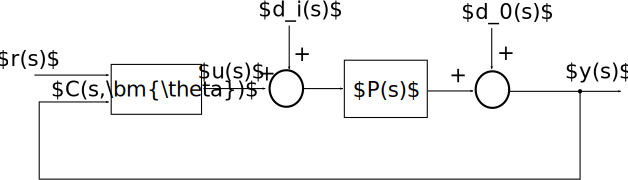
\includegraphics[width=0.8\columnwidth]{Ch4bloques}%pretex=\scriptsize,
	\caption{Feedback control loop.}% 
	\label{fig:bloques}%
\end{figure}
%
Figure~\ref{fig:bloques}, also called closed-loop control system, is designed to keep certain relationship between the process output $y(s)$ and the reference input $r(s)$. For such task, the difference between those signal is used to compute the control signal $u(s)$ needed in order to achieve $y(s)=r(s)$. 

In Figure.~\ref{fig:bloques}, $C(s,\bm{\theta})$ is the \gls{2dof} \gls{pid} controller with parameters:
\begin{equation*}
\bm{\theta}=\left[	\begin{tabular}{cccc} \gls{kp} & \gls{ti} & \gls{td} & \gls{beta}	\end{tabular}\right]^T
\end{equation*}
%
with \gls{kp} the proportional gain, \gls{ti} the integral time constant, \gls{td} is the derivative time constant, \gls{beta} the weight on the reference signal. \gls{plan} represents the controlled process, modeled as a \gls{soptd} plant, with a transfer function of the form:
\begin{equation}  %inclusión de ecuaciones
P(s) =  \frac{K e^{-Ls}}{(T s+1)(a T s+1)},
\label{eq:plantaX}
\end{equation}
%
where \gls{k}, \gls{l} and \gls{t}, correspond to the static gain, the time delay and main time constant respectively. The other pole of the system is represented with a time constant that is fraction of $T$, therefore $0 \leq a \leq 1$. \gls{di} represent the input disturbance while \gls{do} is the output disturbance.

%El diagrama de bloques de un controlador PI de dos grados de libertad se muestra en la Figura \ref{fig:controlador}. 
%
The relationship between the control signal, the reference and the process output is given by:
%
\begin{equation}  %inclusión de ecuaciones
\gls{u} = \gls{contr} \gls{r} - \gls{conty} \gls{y},
\label{us}
\end{equation}
%
where the part applied to the reference signal is given by:
%
\begin{equation}  %inclusión de ecuaciones
\gls{contr}=  \gls{kp}\left({\gls{beta} + \frac{1}{\gls{ti} s}+ \gls{gamma} \frac{\gls{td} s}{\gls{alpha} \gls{td} s +1}}\right),
\label{eq:cr}
\end{equation}
%
and the part applied to the process output is:
%
\begin{equation}  %inclusión de ecuaciones
\gls{conty}=  \gls{kp}\left({1 + \frac{1}{\gls{ti} s}+\frac{\gls{td} s}{\gls{alpha} \gls{td} s +1} }\right).
\label{eq:cy}
\end{equation}

It is common to set $\gls{alpha}=0.1$ and $\gls{gamma}=0$. For this reason, the controller parameter vector is give as $\gls{theta}=[\begin{tabular}{cccc} \gls{kp} & \gls{ti} & \gls{td} &\gls{beta} \end{tabular}]^T$. A detailed depiction of the controller transfer function is presented in 
\begin{figure}[tb]
	\centering
	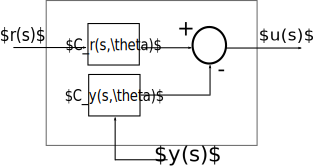
\includegraphics[width=0.8\columnwidth]{Ch4controlador}
	\caption{Representation of the \gls{2dof} controller.}
	\label{fig:Ch4controlador}
\end{figure}
%
Figure~\ref{fig:Ch4controlador}.

To simplify the analysis, the model of the controlled process is normalized:
%
\begin{equation*}
\hat{s}= Ts, \ \tau_0=  \displaystyle\frac{L}{T}, \ \tau_i=  \displaystyle\frac{T_i}{T}, \ \tau_d = \frac{T_d}{T}, \ \kappa_p= K_p K.
\end{equation*}  %inclusión de ecuaciones

Then the normalized parameters of the controller become $\bm{\theta}=\left[\kappa, \tau_i, \tau_d, \beta\right]^T$.
%
and the response of the controlled system is computed as: 
%%
\begin{equation} 
 y(\hat{s})= y_r(\hat{s}) + y_{di}(\hat{s}) + y_{do}(\hat{s}),
\label{ys}
\end{equation}
%
where $y_r(\hat{s})$, is the output response to a change in the setpoint $r(\hat{s})$, $y_{di}(\hat{s})$ is the response to a change in the input disturbance signal $d_i(s)$ and $y_{do}(\hat{s})$ is the response to a change in the ouput disturbace signal $d_o(s)$. From Figure~\ref{fig:bloques} and Figure~\ref{fig:Ch4controlador}, these signals can be computed as:
%
\begin{align*}
 y_r(\hat{s}) &= \frac{P(\hat{s}) C_r(\hat{s},\bm{\theta}) }{1 + P(\hat{s}) C_y(\hat{s},\bm{\theta})} r(\hat{s})\\
y_{di}(\hat{s}) &=  \frac{C_r(\hat{s},\bm{\theta})}{1 + P(\hat{s}) C_y(\hat{s},\bm{\theta})} d_i(\hat{s}) \\%
y_{do}(\hat{s}) &= \frac{1}{1 + P(\hat{s}) C_y(\hat{s},\bm{\theta})} {d_o(\hat{s})}
\label{ytot}
\end{align*}

%Dada \eqref{ys}, la respuesta de salida del lazo cerrado ante un cambio en el valor deseado puede ser ajustada a través del controlador de valor deseado $C_r(\hat{s},\theta)$, independientemente de cambios en la perturbación de entrada o en la de salida. Los parámetros de $C_r(\hat{s},\theta)$ y $C_y(\hat{s},\theta)$ son los mismos con un grado de libertad \cite{apuntescontrol}.

Robustness is an indication of the relative stability of the controlled system and it measure the ability of the controller to keep the closed loop stable despite the variation in the process dynamics. A metric of the degree of relative stability is the maximum sensitivity \gls{ms} given by:
%
\begin{equation}  %inclusión de ecuaciones
\gls{ms}=  \max_\omega \left\{ \frac{1}{\left |{1 + C_y(j\omega ) P(j\omega )}\right |}\right\} 
\label{Ms}
\end{equation}

The recommended value range is  $1.2\leq \gls{ms} \leq 2.0$.

As it is widely established, the controller tuning can be solved as a multi-objective optimization problem~\cite{Gambier2007}. One common indicator of performance, is the \gls{iae} given by:
%
\begin{equation}  %inclusión de ecuaciones
J(\bm{\theta})=\int_0^\infty \left |{e(t,\bm{\theta})}\right | dt.
\label{IAE}
\end{equation}

The error signal $e(t, \bm{\theta})$ it is calculated using:
%
\begin{equation}  %inclusión de ecuaciones
e(t,\bm{\theta})=r(t)-y(t,\bm{\theta}).
\label{error}
\end{equation}

When \eqref{IAE} is computed for a step change in the reference signal, the cost function becomes $J_r(\bm{\theta})$; for an input disturbance response, the function is defined as $J_{di}(\bm{\theta})$ and finally, for an output disturbance response, the cost function is named as $J_{do}(\bm{\theta})$.

When the output of the plant is disturbed only by the step change in $d_i(s)$, the error signal then becomes:
\begin{equation}  %inclusión de ecuaciones
e_d(t)=-y_{di}(t)
\label{per}.
\end{equation}

And then, the cost function $J_{di}(\bm{\theta})$ is computed as:
\begin{equation}  %inclusión de ecuaciones
J_{di}(\bm{\theta})= \int_0^\infty  \left |-{y_{di}(t,\bm{\theta})}\right | dt,
\label{perin}
\end{equation}

On the other hand, if the disturbance comes only from a step signal in $d_o(s)$, the cost function that has to be computed is $J_{do}(\bm{\theta})$ as:
%
\begin{equation}  %inclusión de ecuaciones
J_{do}(\bm{\theta})= \int_0^\infty  \left |-{y_{do}(t,\bm{\theta})}\right | dt.
\label{perout}
\end{equation}	
%

Finally, if the setpoint is the only source of disturbance for the plant, the corresponding cost function $J_r(\bm{\theta})$ is computed as:
\begin{equation}  %inclusión de ecuaciones
J_r(\bm{\theta})=\int_0^\infty \left |r(t)-y_r(t,\bm{\theta})\right | dt.
\label{eq:Jr}
\end{equation}
%

In general, it is not possible to optimize $\bm{\theta}$ for those three functions at the same time. Such impossible point where all the cost functions are optimal is called Utopia point, but optimizing one of them always produce a degradation in the other remaining functions. All the solutions that are closest to the utopia point, create the Pareto frontier which, if all cost functions are considered equal, are equally optimal. 

The problem of minimizing $J_r(\bm{\theta})$, $J_{di}(\bm{\theta})$ and $J_{do}(\bm{\theta})$ at the same time can be posed as a \gls{moo} problem. In addition, since in an industrial environment the robustness is very important, the obtained parameters are constrained to always satisfy  $\gls{ms} \leq M_{s,max}$, where $M_{s,max}$ is the allowed limit of the maximum sensitivity. The combined cost function (vector of cost functions) then becomes:
%
\begin{equation}  %inclusión de ecuaciones
\textbf{J}(\bm{\theta})=\left[J_{di}(\bm{\theta}), J_{do}(\bm{\theta}), J_{r}(\bm{\theta})\right]^T,
\label{eq:Jtotal}
\end{equation}
%
and solved by finding all possible optimal solutions of:
%
\begin{equation}  %inclusión de ecuaciones
\begin{gathered}
\textbf{J}(\bm{\theta}^*) = \min_{\bm{\theta}} \textbf{J}(\bm{\theta}),\\
\text{s.t.} \quad  M_s \leq M_{s,max}
\end{gathered}
\label{eq:probmoo}
\end{equation}

\textbf{To do: Expand more this part}
\chapter{Multi-objective optimization}
\label{sec:Metodolgia}
%\begin{refsection}

\abstract{Before tackling the problem of multiple criteria for \gls{pid} tuning, the multi-objective optimization is explained in general. First the basic formulation of the optimization problem is presented with the introduction of the Pareto front concept. The methodology chosen to solve the multi-objective optimization problem is to transform the multi-criteria situation into a single scalar cost function. However it is known that this scalarization procedure may not yield to a good Pareto front. For this reason several scalarization methods are presented and compared. The Pareto found using this scalarization methods may be used as just data that can be later used or may be directly used as part of a decision tool useful to select the final solution to the problem.} 

\section{Formalization of the multi-objective optimization problem}
\label{sec:MOOPForm}
%
A \gls{moop} arises when, in order to solve a given problem or design, it is necessary to optimize several cost functions at the same time. 

In general, these cost functions depend on the same variables and usually are in conflict.  In addition, they may be independent of one another, that is, the value of the variables that optimize one of the function do not necessarily optimize the other cost functions.

In those cases, given a set of cost functions:
\begin{equation}
\mathbf{F}(\xv)=\left[F_1(\xv), F_2(\xv), F_3(\xv), \ldots, F_k(\xv)\right]^T
\label{eq:functions}
\end{equation}
%
that depends on $n$ different variables $\xv=\left[x_1, x_2, \ldots, x_n \right]^T$, $x_i \in \mathbf{X}$, where $\mathbf{X}$ is the feasible decision space. The \gls{moop} may be formulated as follows \citep{Marler2004}:%
%
\begin{subequations}%
	\begin{align}%
	&\min_\xv \mathbf{F}(\xv), \label{eq:Min01}\\ %
	&\text{s.t.}\nonumber\\%
	& \hspace{5mm} g_j(\xv) \leq 0, \qquad j=1,2,\ldots,m  \label{eq:Min02}\\ %
	& \hspace{5mm} h_l(\xv) = 0, \qquad l=1,2,\ldots,e  \label{eq:Min03}%
	\end{align}%
	\label{eq:OptProb}%
\end{subequations}%
%
where $g_j(\xv)$ is the $j$-th inequality constraint and $h_l(\xv)$ is the $l$-th equality constraint. 
%
\subsection{Definition of the Pareto front}
In general, it is not possible to find a set of variables values that minimizes all $F$ functions. In fact, the optimization problem in \eqref{eq:OptProb} have multiple equally optimal solutions in the sense of the Pareto optimality. According to \citet{Marler2004}:
\begin{quote}
	``A point $\xv^*\in \mathbf{X}$, is Pareto optimal iff there does not exist another point, $\xv \in \mathbf{X}$, such that $\mathbf{F}(\xv)\leq\mathbf{F}(\xv^*)$, and $F_i(\xv)<F_i(\xv^*)$ for at least one function''
\end{quote}

The concept of Pareto optimality is represented in %
%
\begin{figure}[tb]
	\centering
	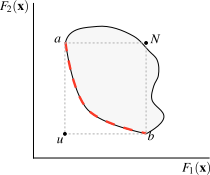
\includegraphics[width=0.8\columnwidth]{Ch5planoFun01}
	\caption{All possible solutions and the Pareto front in the function space.}
	\label{fig:planoFun01}
\end{figure}
%
figure~\ref{fig:planoFun01} for a two-function multi-objective optimization. The gray area represents the feasible function space, given by the value of $F_1(\xv)$ and $F_2(\xv)$ for all $\xv \in \mathbf{X}$. From all those points, only the points in the curve from ``a'' to ``b'' (marked with a thicker dash line) are Pareto optimal because there is not another point in the feasible decision space with a lower value of $\mathbf{F}$, but there is at least one point that has a lower value for either $F_1$ or $F_2$. The curve from ``a'' to ``b'' is the Pareto front and contains all possible solutions to problem \eqref{eq:OptProb} that are Pareto optimal. These solutions are always in the edge of the feasible function space, closer to the utopia point (the ``u'' point in the figure). The utopia point is a point in the space where all the cost functions have their minimum value. As it can be seen from figure~\ref{fig:planoFun01}, this point is more likely to be outside of the feasible function space.

Points ``a'' and ``b'' are called anchor points and represent the combination of decision variables that optimizes at least one of the functions. In this case, ``a'' is the point where function $F_1(\xv)$ has its minimum value whereas ``b'' the one in which $F_2(\xv)$ has its minimum value.

Point ``N'' is called the pseudo-nadir point, and is defined as the point with the worst values of all the anchor points.
\subsection{Different approaches to obtain the Pareto front}
In its most basic form, the Pareto front is found by performing several optimizations, each of which are computed by varying some parameter. The idea is to be able to use standard optimization methods to find each point of the Pareto.

As for single objective optimization there is two big families of methods to solve the problem: Bio-inspired methods that use some kind of heuristic in order to find the minimum of the cost function and deterministic methods mostly based on certain gradient of the function.

In this section, a short review on both families is presented. However, because of the deterministic nature of the gradient based methods, in this book the later family is chosen tool for solving \gls{moop}.
%
In \citet{Zhou2011} a review on multi-objective evolutionary algorithm is presented. The author indicates that several of the algorithms are similar to the non-dominated sorting genetic algorithm II (NSGA-II) \citep{Deb2002}. Genetic algorithms are based in the idea of random mutation across generations and interchange of genes from parents to children. They also explain other kind of algorithms like particle swarm optimization which is based on the social behavior of bird flocking or fish schooling \citep{Eberhart1995}. Originally this method was employed for single function optimization, but it has been extended for multiple cost functions. Other methods that has been used for solving \gls{moop}, have a probabilistic nature like Ant Colony Optimization \citep{Dorigo2005} or the Cross Entropy method \citep{Rubinstein2004}. One drawback is that these methods are heuristic, and may yield different results each time they are computed. However, the main advantage is that they probably are able to find the global minimum of the functions.

Specifically, for \gls{pid} control, evolutionary algorithms have been used in \citet{Reynoso-Meza2012b} for the multivariate process of the Wood and Berry distillation column. Another case is presented in \citet{Pierezan2014} where multi-objective Particle Swarm Optimization is applied on multivariable PID controllers tuning to improve the performance of a robotic manipulator. This method was also used in \citet{Tian2014} but applied to a nonlinear process continuous stirred tank reactor. In a general process control case, in \citet{Cespedes2016} Ant Colony Optimization, Invasive Weed Colony Optimization \citep{Mehrabian2006}, Linear Biogeography-based optimization \citep{Simon2008}, Genetic Algorithms and Particle swarm optimization are compared when solving the tuning of an industrial \gls{pid} controller for \gls{soptd} plants.

Also in \citet{Mahdavian2014}, a multi-objective optimization for \gls{pid} control of a greenhouse electrical lighting system based on the cost of electricity is investigated and solved using an evolutionary algorithm. Multiobjective salp swarm algorithm (MSSA) with opposition based learning initialization and evolution was used in \citet{Domingues2019} for tuning the parameters of a \gls{pid} controller for an Antilock Braking Systems with good results over NSGA-II, but the later was more consistent with the results.

In the other hand, the deterministic methods are primarily based on a scalarization method. The main idea is to take all the cost functions and formulate the problem in such a way that can be readily solved using an standard optimization method. The main methods are the \gls{ws} \citep{Marler2004}, the \gls{nbi} \citep{Das1998}, the \gls{nnc} \citep{Messac2003} and the \gls{ennc} \citep{Sanchis2008}. These methods are explored in the next section and used in the rest of the book.
%----------------------------------------------------
\section{Scalarization algorithms to find the Pareto front}
\label{sec:design-methodologies}

In general, the algorithms to find the optimal value of a function are designed to be used in a single objective paradigm. In order to be able to use the same standard algorithms with a multi-objective problem, some scalarization method has to be employed.
%
\subsection{Weighted Sum}
\label{sec:WS}
\gls{ws} methodology is a popular procedure to transform a \gls{moop} into a single objective problem by creating a new objective function that is the result of the aggregation of all the functions involved with certain weight for each one \citep{Marler2004}:
%
\begin{equation}
F_{WS}(\mathbf{x}) = \sum_{i=1}^{k}\alpha_{i} {f}_{i}(\mathbf{x}),
\label{eq:JWSOriginal}
\end{equation}
%
where $\alpha_i$ is the weight of associated with function $f_i$. The idea behind the utility function $F_{WS}$ is to be able to take into account all individual cost functions at the same time. It is known that when minimizing \eqref{eq:JWSOriginal}, the solution belongs to the Pareto front. Therefore, it is of great importance to select the values of the weights that better reflect the desire of the decision-maker.

The weights have two different roles that are entangled, in one hand the weights can be used to represent the importance of one function over the others (the bigger the weight, the higher the importance) and in the other hand the weights ca be used to equalize the relative values of the functions (one function may yield higher values that shadows the others).

However, choosing the values of the weight can be difficult. In \citet{Marler2010} it is shown that the weight can be interpreted as a first order approximation of a preference function, and therefore, cannot fully take into account the desires of the decision-maker.

Lets take a two function \gls{moop} as an example. If the Pareto front wants to be computed, one may try to first normalized the function:
\begin{equation}
F_{WS}(\mathbf{x}) = \alpha_{1WS} \hat{f}_{1}(\mathbf{x}) + \alpha_{2WS} \hat{f}_{2}(\mathbf{x}),
\label{eq:JWS}
\end{equation}
with $\alpha_{1WS} + \alpha_{2WS}=1$, and $\hat{f}_{1}(\mathbf{x})$ and $\hat{f}_{2}(\mathbf{x})$ the normalized versions of $f_{1}(\mathbf{x})$ and $f_{2}(\mathbf{x})$, respectively. One possible normalization (see \citet{Marler2004}) is given by:
\begin{equation}
\hat{f}_{1}(\mathbf{x}) = \frac{f_{1}(\mathbf{x})-\min{\left( f_{1}(\mathbf{x})\right) }}{\max{(f_{1}(\mathbf{x}))}-\min{\left( f_{1}(\mathbf{x})\right) }}.
\label{eq:NormalizedJ}
\end{equation}

With this normalization, the utopia point is moved to the origin and the maximum value of the new normalized function is 1.

The optimization problem then is written as:
\begin{equation}
\begin{gathered}
\min_{\mathbf{x}}{\; F_{WS}(\mathbf{x})}, \\
\text{s.t.} \; h(\mathbf{x})=0, \\
g(\mathbf{x}) \leq 0,
\end{gathered}
\label{eq:WSProblem}
\end{equation}
%
where $h(\mathbf{x})$ and $g(\mathbf{x})$ are the equality and inequality constraints of the original problem. To find the Pareto front, the problem in \eqref{eq:WSProblem} is solve varying the weights. However, it is known that the \gls{ws} method is not appropriate to find the Pareto front. In first place, when \eqref{eq:JWS} is minimized for different values of $\alpha_{1WS}$ and $\alpha_{2WS}$ in order to obtain the Pareto front, an even distribution of the weights does not assure an even distribution of the points in the front. Also, with \gls{ws} it is not possible to obtain Pareto points in the non-convex region of the front, and therefore, not all the possible solutions can be found \citep{Das1997}. In order to tackle this issue, alternative problem formulation have been proposed in the literature to obtain the Pareto front which are presented next.
%--------------------------------------------------
%--------------------------------------------------
\subsection{Normal Boundary Intersection}
\label{sec:NBI}
%
The \gls{nbi} is a variation in the way that the \gls{moop} is posed as a single objective optimization problem, in order to obtain an even spaced Pareto front \citep{Das1998}. In %
%
\begin{figure}[b]%
	\centering
	\includegraphics[width=0.8\columnwidth]{Ch5NBI}%
	\caption{\gls{nbi} optimization method.}%
	\label{fig:NBI}%
\end{figure}
%
figure~\ref{fig:NBI}, a representation of the method is shown for two normalized objective functions. If the utopia plane (the plane that contains the anchor points, in the case of a bi-objective problem, the straight line that joins the anchor points) is parameterized by $\Phi\mathbf{\beta}$, where $\Phi(:,i)=\mathbf{F}(\mathbf{x}_i^*)-\mathbf{F}(\mathbf{x}^*)$, $\mathbf{F}(\mathbf{x}_i^*)$ is the value of the multi-objective function evaluated in the $i$th anchor point, $\mathbf{F}(\mathbf{x}^*)$ is the value of the function at the utopia point, and $\beta$ is chosen as:
\begin{equation}
\beta=
\left[\begin{tabular}{c}
$\alpha_{1NBI}$ \\ $\alpha_{2NBI}$
\end{tabular}\right],
\label{eq:Beta}
\end{equation}
with $\alpha_{1NBI}+\alpha_{2NBI}=1$.

The central idea behind the \gls{nbi} method is to find the maximum distance from the utopia plane towards the utopia point (with direction $\hat{\mathbf{n}}$) that is normal (or quasi normal as proposed in \citet{Das1998}) to the utopia plane. In other words, this method finds the border of the feasible region that is closer to the utopia point (farther from the utopia plane). This problem is considered a subproblem, because with one given $\beta$,only one point of the Pareto front is found but, by varying this parameter $\beta$ evenly, it is possible to obtain an even spaced realization of the front.

The problem then is posed as follows:%
%
\begin{equation}
\begin{gathered}
\max_{\xv,v}{\;v}, \\
\text{s.t.} \ \Phi \boldsymbol{\beta} + v \hat{\mathbf{n}} = \mathbf{F}(\xv),\\
h(\xv)=0, \\
g(\xv) \leq 0.
\end{gathered}
\label{eq:NBIProblem}
\end{equation}%

The \gls{nbi} method converts the original problem by adding an equality constraint. By maximizing the new variable $v$ (which represents the distance from the utopia plane towards the utopia point), the front that is closer to the utopia point is found. An alternative formulation of \eqref{eq:NBIProblem} was proposed in \citet{Shukla2007} to ensure that only the points that really belongs to the Pareto front are found.

This method has been widely used in several areas.For example, in \citet{Stehr2003} was used to analyze the compromise between gain and phase margin when designing analog circuits. In \citet{Sendin2004}, the \gls{nbi} was considered in the design of nonlinear bioprocesses. In \citet{Ierapetritou2007a} the \gls{nbi} is used to optimize the scheduling of a chemical process with uncertainty. In \citet{Vahidinasab2010} \gls{nbi} is applied to develop optimal bidding strategies for the participants of oligopolistic energy markets; the social welfare and the emissions are considered as the cost functions and the constraints take into account the characteristics of the generators and the power flow of the system. In \citet{Ganesan2013}, \gls{nbi} is used in conjunction with a meta-heuristic algorithm to generate optimal solution options to the green sand mould system problem. In \citet{Brito2014} the method is used coupled with mean-squared error functions in a robust parameter design of the surface roughness in end milling process. In \citet{Rubio-Largo2014} the method is adapted to solve a traffic grooming problem in the telecommunication field. In \citet{Rojas2015b} a comparison between several scalarization methods, including \gls{nbi}, was presented for a \gls{foptd} plant where different disturbance sources are considered. In \citet{Naves2017} \gls{nbi} is used for the optimization of methyl orange treatment with ozone. In \citet{Simab2018} a model for short-term hydrothermal scheduling problem in the presence of the pumped-storage technology and stated as Mixed-Integer Non-Linear Programming, while the scalarization was done using \gls{nbi}. Finally, in \citet{Moura2018} \gls{nbi} was used in the construction of a Pareto boundary chart of a treatment of a synthetic solution of amoxicillin in a reactor with ozone bubbling.
%-------------------------------------------------- 
\subsection{Normalized Normal Constraint}
\label{sec:NNC}
The \gls{nnc} is presented in \citet{Messac2003} and is intended to improve the results of the \gls{nbi} by formulating the optimization problem only with inequality constraints and by filtering all the non-Pareto optimal points. The main idea of the methodology is presented in
%
\begin{figure}[b]%
	\centering
	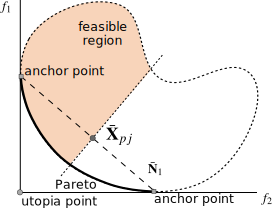
\includegraphics[width=0.8\columnwidth]{Ch5NNC}%
	\caption{NNC optimization method.}%
	\label{fig:NNC}%
\end{figure}
%
figure~\ref{fig:NNC}: the utopia plane is parameterized in a similar way as the \gls{nbi} but, instead of constraining the points to be within a line, the new constrained feasible region is constructed with the original feasible region and a line that is normal to the utopia plane. With this new feasible region it is only required to minimize one of the functions (e.g. $f_{1}$) in order to find the Pareto front.

By varying the parameter $\bar{\mathbf{X}}_{pj}$ along the utopia plane, it is possible to find an even spaced front. $\bar{\mathbf{X}}_{pj}$ is computed as%
%
\begin{equation}
\bar{\mathbf{X}}_{pj}= \alpha_{1NNC} \mathbf{\hat{F}}(\mathbf{x}_1^*)+\alpha_{2NNC} \mathbf{\hat{F}}(\mathbf{x}_2^*).
\label{eq:Xpj}
\end{equation}%
%
with $\alpha_{1NNC}+\alpha_{2NNC}=1$ and where $\mathbf{\hat{F}}(\mathbf{x}_1^*)$ is the first anchor point and $\mathbf{\hat{F}}(\mathbf{x}_2^*)$ is the second. The methodology can be extended to higher dimensions.

The optimization problem can be written as follows:
%
\begin{equation}
\begin{gathered}
\min_{\mathbf{x}}{\; \hat{f}_{1}(\mathbf{x})}, \\
\text{s.t.} \ \bar{\mathbf{N}}_1^T \left(\hat{\mathbf{F}}(\mathbf{x})-\bar{\mathbf{X}}_{pj}\right) \leq 0,\\
h(\mathbf{x})=0, \\
g(\mathbf{x}) \leq 0,
\end{gathered}
\label{eq:NNCProblem}
\end{equation}
%
where $\bar{\mathbf{N}}_1$ is the vector that contains the direction of the utopia plane. In some cases, the optimization may yield points that do not belong to the Pareto front. In \citet{Messac2003}, the authors propose to use a filter algorithm to eliminate those points.

This method has been used in several cases. Also in \citet{Hosseini2016a} the method was implemented to optimally solve the transmission congestion management taking into account the cost of congestion management, voltage stability margin, and transient stability margin. In \citet{Sanchez2017a}, the \gls{nnc} was considered to find optimally balanced tuning rules for fractional-order proportional-integral-derivative controllers for \gls{foptd} process models subject to a robustness constraint. In \citet{Mittal2017a} the NNC was used in conjunction with an evolutionary algorithm to find the optimum number and location of wind turbines in a wind farm. In \citet{Benki2018}, the \gls{nnc} was implemented in the design of an aerosol can, tanking into account both the dome growth and the dome reversal pressure DRP. In \citet{Tan2018a}, the \gls{nnc} was applied in the design of microvascular panels for battery cooling applications. The NNC is also applied in \citet{Liu2019} within their algorithm to optimally control the glycerol in a 1,3-propanediol batch process.

\subsection{Enhanced Normalized Normal Constraint}
\label{sec:ENNC}
The \gls{ennc} \citet{Sanchis2008}, is a new perspective of the original \gls{nnc} method. Implicitly, the \gls{nnc} method supposes that in each anchor point, the other functions that are not optimal, have their worst value. For a two functions optimization, this is always the case; however for more than two functions this supposition is not true in general. The \gls{ennc} method redefines the anchor points in such a way that the supposition of the \gls{nnc} holds true, and then the same method may be used. Other advantage of the \gls{ennc} is that it is possible to expand the explored regions of the problem, given a better representation of the Pareto front.
%
The new anchor points (called pseudo anchor points) are defined as:
\begin{equation}
F_i^{**} = \left[
\begin{tabular}{cccccc}
$f_1^N$ & $f_2^N$ & $\cdots$ & $f_i^{*}$ & $\cdots$ & $f_n^N$
\end{tabular}
\right],
\label{eq:PseudoAnchor}
\end{equation}
%
where $f_i^N$ if the value of function $f_i$ at the pseudo nadir point. The effect of this new definition is to enlarge the utopia hyper plane and scaling the functions in such a way that the Pareto front is evenly obtained while the unexplored regions of the Pareto are reduced.

The Pareto is then computed using the same methodology as in the \gls{nnc} case. This method has also been applied in several cases, for example in \citet{Contreras-Leiva2016}, the \gls{ennc} is applied in the optimization of the tuning parameters of a \gls{2dof} \gls{pid} controller for an \gls{soptd} plant. In\citet{Pereira2017b} an augmented version of the \gls{ennc} is applied to optimized the milling process of aluminum alloy Al 7075 taking into account the axial cutting force, the energy consumption and the material removal rate. The \gls{ennc} is tested in the optimization of a multiobjective model based predictive controller and compared with different techniques in \citet{Toro2011} and for the nonlinear case in \citet{Vallerio2014}.
%--------------------------------------------------
\section{Solution selection from the Pareto front}
\label{sec:Selection}
%%--------------------------------------------------------------------------
%%-------------------------------o-o-o--------------------------------------
%%--------------------------------------------------------------------------
The optimizations techniques presented in Section~\ref{sec:design-methodologies} are very well suited to find the Pareto Front of a multiobjective optimization problem. However, in the end, it is necessary to decide which of the multiple equally optimal points is the one that is going to be selected as the final solution.

Consider the general Pareto Front presented in 
\begin{figure}[b]
	\centering
	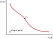
\includegraphics[width=0.8\columnwidth]{Ch5GeneralPareto}
	\caption{General Pareto Front with one solution selected.}
	\label{fig:Ch5GeneralPareto}
\end{figure}
%
Figure~\ref{fig:Ch5GeneralPareto}. Once the Pareto is computed, it is certainly very useful to plot it to see how the cost functions $f_1(\mathbf{x})$ and $f_2(\mathbf{x})$ vary with the change in the decision variables $\mathbf{x}$. In this figure, the arbitrary solution $p_1$ is pointed out. By definition, all points in the Pareto Front are equally optimal, therefore, what makes $p_1$ any special from other points? More important, how any of the Pareto points can be selected from any other?

One may then conclude that obtaining the Pareto front is half the solution to the \gls{moop}. The final task to fully solve the problem is to be able to select one of the (maybe infinite) possible points of the Pareto. With a front like the one presented in Figure~\ref{fig:Ch5GeneralPareto}, it may be easy to explore all possible solutions, but with more than three objective functions, it is impossible to directly plot the front. And even with three objectives, the visualization of the results may be cumbersome.

Even more, the plot of Figure~\ref{fig:Ch5GeneralPareto} contains the solutions viewed from the function space, but what is really necessary is to know the value of the decision variables. But each of every point in the Pareto is associated with a $n$-size vector representing one of the optimal solutions. Once again, plotting the Pareto is not enough to help the decision maker to solve the problem.

For these reasons, once the Pareto is found, it may be useful to accomplish some tasks to help the decision maker:
\begin{itemize}
	\item  Visualize the Pareto to understand the relation between the cost functions and the decision variables.
	\item Use the Pareto as data for the construction of a decision tool.
	\item Use the Pareto as part of a decision tool.
\end{itemize}
In the following, these three tasks are going to be explored.
%
\subsection{Visualization of the Pareto Front}
\label{sec:ParetoVisualization}
%
One of the advantages of using a multiobjective problem approach, is its ability to take into account many cost functions at the same time, and being able to find the set of the \emph{best} solutions. This is the ultimate goal of a multiobjective optimisation, to provide useful information to the decision makers in order to help to choose according to its preferences. This can be done in terms of a large set of raw data that has lately to be processed accordingly. This introduces some cognitive issues that become harder and a clear obstacle for decision making stage, especially when having many objectives (say more than 3). Although there are some performance metrics that can evaluate the quality of a Pareto front approximation set (Inverted Generational Distance \citep{Bosman2003} and Hypervolume \citep{Zitzler1999} among others), it is still not intuitive this approach really helps the decision maker to understand the trade-off relationship among objectives.

In contrast, high-dimensional data visualisation is a widely recognised effective way to facilitate the analysis and understanding of multidimensional data. more effective and intuitive to facilitate the decision maker stage to understand the trade-off solutions and thus make a meaningful decision. In the context of multi-objective optimisation, comparing to quantitative performance metrics, visualisation is, in principle, able to provide a decision maker better insights about Pareto front approximation sets (e.g. the distribution of solutions, the geometric characteristics of Pareto front approximation) thus to facilitate the decision-making (e.g. the exploration of trade-off relationship, the knee region or region of interest).

According to \citet{Gao2019} a high quality visualisation tool must provide three types of information in the high dimensional space. 
\begin{itemize}
\item  Should provide accurate shape, location, and range of the approximate Pareto front. 
\item  From the provided visualisation, decision makers can observe trade-off between objectives, monitor the evolution progress, assess the quality of the approximate front, and select their preferred solutions if desired. 
\item  Should be scalable to any dimensions, handle a large number of individuals on the approximate front, and simultaneously visualise multiple fronts for the purpose of visual comparison. Moreover, the resulted visualisation plot should be robust and insensitive to the addition or removal of an individual.
\end{itemize}

To tackle these issues, different kinds of plots have been proposed in the literature that tries to present all the information of the Pareto in a bi-dimensional graph. Generally speaking, they can be divided into three categories. Interested readers are encouraged to found a recent taxonomy from \citet{B.2018}.

\begin{description}
\item [A. Visualisation of All Objective Information] These visualisation techniques aim to reveal all individual objective information of the underlying approximation set. Specifically, scatter plot is the most commonly utilised data visualisation technique that provides a holistic exploration of the population distribution. 

\item [B. Visualisation via Dimension Reduction] Techniques in this category aims to transform the high-dimensional data into a lower dimensional space to facilitate the human cognition. In modern data analytics, there are many dimension reduction techniques available to implement such transformation.  Instead of using dimension reduction techniques from machine learning, In \citet{Blasco2008}, Blasco et al. proposed a new visualisation technique called level diagrams to visualise the approximation set in a objective-wise manner. More specifically, each diagram is a two-dimensional scatter plot where the horizontal coordinate represents the objective value at the corresponding objective while the vertical coordinate indicates the distance with respect to the ideal point. As claimed by the authors, the level diagrams are able to facilitate the investigation of some of the Pareto front characteristics, i.e. discontinuities, closeness to ideal point and ranges of attainable values. 

\item [C. Visualisation via a Transformed Coordinate System] Techniques in this category share some similarity with the dimension reduction. They also aim to visualise the original high-dimensional data in a lower-dimensional space. But they try to maintain the original information as much as possible. For example, Ibrahim et al. \citet{Ibrahim2016} developed a variant of the classic Radial coordinate visualisation (RadViz) \citep{Hoffman2002}, called 3D-RadViz, by adding an additional dimension. In particular, this additional dimension represents the perpendicular distance between a solution and a hyper-plane formed by the extreme points of the underlying population. By doing so, the 3D-RadViz is able to provide the information of the convergence of the population. 
\end{description}

As usual when there do exist different approaches to deal with a complex problem, there is  no single visualisation technique is able to provide a comprehensive understanding of the characteristics of the approximation set. It is important to know the specific characteristics, pros and cons of each approach and evaluate the suitability for the problem at hand.
  
\subsection{The Pareto as a decision tool}
\label{sec:ParetoData}
%
Since the Pareto front cannot be considered as the final solution of the \gls{moop}, one may use it as the basis to construct a tool that takes advantage of the multiple optimal points found.

In other words, the Pareto front becomes the raw material that is used to produce the final decision tool. This tool may be an algorithm (as a tuning rule for PID controllers for example) that incorporates the information obtained from the optimization to produce a final decision.

For example in \cite{Zhao2007}	the concept of Pareto optimality is used to define a genetic programming approach for optimal decision trees. The author presented a Java code for the final tool and use code in two different study cases.

Another example can be found in \cite{Das2012}. In this paper, the route for the transportation of hardzarous waste has to be selected taking into account the cost of the route and the mortality and morbidity of incidents. Once the Pareto frontier has been obtained, the authors present a selection criteria where the Cost Elasticity of risk and the Knees on the Pareto are taken into account for the final decision.
%
%\subsection{The Pareto Front as part of a decision tool}
%\label{sec:ParetoDecision}
%\textbf{To do}
%
\bibliographystyle{spbasic}
\bibliography{ReferenciasMulti}
\chapter{PID tuning as a multi-objective optimization method}
\label{chap:PIDMOOP}
\section{Formalization of PID tuning as a multiobjective optimization problem}
\label{sec:FormPIDMOOP}
To do
\subsection{Cost functions and constraints selection}
\label{sec:CostFunSelec}
To do
\subsection{PID tuning problem formulation for integral cost functions}
\label{sec:CostProbPID}
To do
%-----------------------------
\section{Solution of the multi-objective optimization tuning}
\label{sec:SolMOOP}
To do
\subsection{Database approach for the final tuning}
\label{sec:DatabaseMOOP}
To do
%
\subsection{Viability for tuning rules}
\label{sec:TuningRulesMOOP}
To do
\chapter{Application examples}
\label{chap:ApplicationExamples}
%
%
In this chapter different examples are going to be used as exploration ground for the \gls{moo} framework for \gls{pid} tuning. In Section~\ref{sec:Bechmark} the \gls{ennc} method is applied in a typical high order benchmark plant. Then in Section~\ref{sec:LiTAO3}, the framework is tested with a the temperature control in a deposition process of lithium tantalate (LiTaO$_3$) which has a important dead-time. Finally, the MOOTuning software is used to analyze the temperature control in a Continuous Stirred Tank Heater in Section~\ref{sec:CSTH}.

\section{High order benchmark plant}
\label{sec:Bechmark}
First the \gls{ennc} method is going to be tested in high order benchmark plant \cite{Astroem2000}. The model of the plant is given by a fourth order transfer function:
\begin{equation}
P(s) = \frac{1}{\prod_{n=0}^{n=3}(0.5^n s+1)}.
\label{eq:benchmarkTF}
\end{equation}

The first step is to obtain a low order model that is able to reflect the main dynamics of the plant. In general, the tuning of \gls{pid} controllers starts with a first or second order model \cite{Alfaro2006}. In this particular case, using a step change as the input signal, the low order model that can be found from this experiment is given by:
%
\begin{equation}
F(s)=\frac{e^{-0.297s}}{(0.9477s+1)(0.6346s+1)},
\label{eq:BenchTFfit}
\end{equation}
%
alternatively, if it is supposed that the ``real'' model of the plant is known, an order reduction procedure, for example, the half-rule method \cite{Skogestad2003} may be used. The comparison between the high order model and the reduced order model in the time domain is presented in %
\begin{figure}[tb]
	\centering
	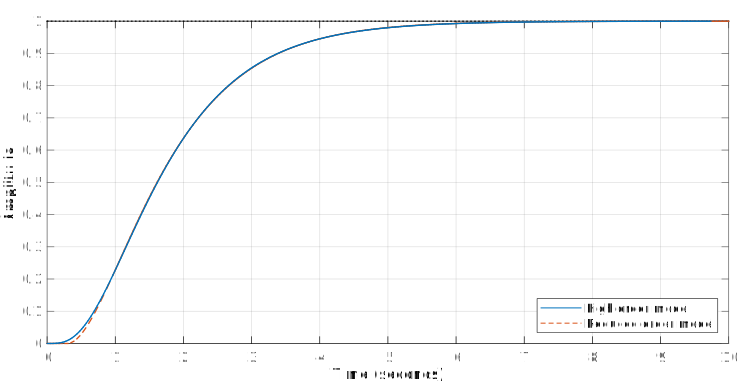
\includegraphics[width=0.9\columnwidth]{Ch7CompRespBench}
	\caption{Comparison between the high and reduced order models.}
	\label{fig:Ch7CompRespBench}
\end{figure}
%
Figure~\ref{fig:Ch7CompRespBench}. As it can be seen, the model represent accurately the dynamics of the original plant and therefore is considered to be a good approximation of the original model.

The next step is to find the Pareto front for this particular plant. The followed methodology was as presented in Chapter~\ref{chap:PIDMOOP}. For this particular case, only $J_{di}$ and $J_r$ where considered as the cost functions with a \gls{2dof} \gls{pid} controller. In Figure~\ref{fig:paretomodelo}, the obtained Pareto front is presented. 
%^
\begin{figure}[tb]%
	\centering
	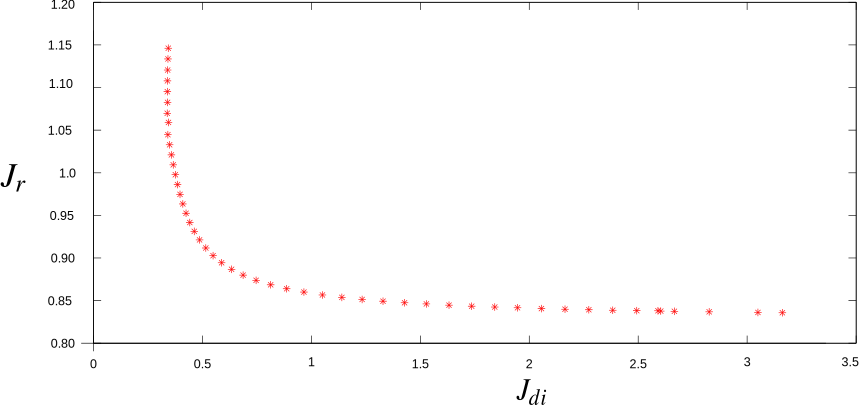
\includegraphics[width=0.9\columnwidth]{paretomodelo}%
	\caption{The Pareto front for the benchmark process.}%
	\label{fig:paretomodelo}%
\end{figure}

The curve has a typical form, with a high slope for low values of $J_{di}$ and an almost flat slope for higher values. This shape has a particular physical meaning: to improve the response of the $J_{di}$ cost function, the $J_{r}$ value has to be augmented (worsening the servo response), however the degradation is not as much as the improvement in the $J_{di}$ function. This is a clear example of one of the many advantages of using a multi-objective framework for controller tuning and the main reason why is the chosen framework in this book, it gives the decision taker more tools to select the more appropriate tuning for the controllers.

In order to compare the response of the optimal controllers, the tuning for the anchor points are presented along the resposes of the ART$_2$ method \cite{Vilanova2011} and the uSORT$_2$ method\cite{Alfaro2012a}, in order to compare the performance of the closed loop response. It is important to clarify that these two tuning are just the extreme points of the Pareto front, thanks to the ENNC method and that there is a practically and infinite amount of possible parameter tuning to select. The obtained parameters are listed in %
%
%parámetros del controlador
\begin{table}[tb]
	\caption{PID controller parameters using two degrees of freedom.}
	\centering
	\begin{tabular}{@{}*{5}{c}@{}}
		\toprule
		Tuning              &$K_c$       &$T_i$      &$T_d$     & $\beta$ 	\\
		\midrule              
		optimum $J_{di}$     &$3.3750$   & $1.0812$  &$0.3095$  &$0.5466$   \\
		optimum $J_{r}$      &$3.0572$   & $8.4419$  &$0.3986$  &$1.2329$   \\
		$ART_2$             &$3.3657$   & $1.7636$  &$0.4884$  &$0.2971$   \\
		$uSORT_2$           &$3.1708$   & $0.8997$  &$0.3945$  &$0.4731$   \\	
		%
		\bottomrule				
	\end{tabular}
	\label{tab:parametroscontrolador}
\end{table}
%
Table~\ref{tab:parametroscontrolador} for reference. It is important to note that in all cases, the Maximum Sensibility was set to be around $M_s = 2.0$ to ensure a minimum level of robustness.

In Figure~\ref{fig:Ch7cambioreferencia}, the closed-loop responses of all the four controllers are presented for the case of a step change in the setpoint. it was found that precisely the controller in the anchor point of the Pareto front that give the minimum value of $J_r$ is in fact the one that give the best result of all the controllers. However, it has to be noticed that both ART$_2$ and uSORT methods are intended for regulator response mainly, and theredore, it was not expected to have a low $J_r$. The obtained values are given in Table~\ref{tab:IAEref} where both the \gls{iae} and \gls{ms} are presented. 

On the other hand, the optimal controllers in the regulator mode are presented in Figure~\ref{fig:cambiodi}. Again, as expected, the controller in the anchor point that has the lowest value of $J_{di}$, is the one with the fastest response. Also, it is clear that the other anchor point (the one with the lowest value of $J_r$) has the worst response for disturbance rejection as it was expected. In table \ref{tab:IAEdi}, the corresponding values of IAE for the curves in Figure~\ref{fig:cambiodi} are presented.

The optimal controller for disturbance rejection is presented in figure \ref{fig:cambiodi}. Again, the tuning given by the ENNC method is the fastest response to reach the desired value. As it can be seen, the ART$_2$ and the uSORT$_{2}$ methods fall between these two optimal responses. However, it does not necessarily means that these methods are optimal because they could be dominated by other controllers that are exactly in the front. Only the tuning found with the ENNC method can be considered to be Pareto optimal using the \gls{iae} as the metric. In Table~\ref{tab:IAEdi}, the IAE values of the responses presented in Figure~\ref{fig:cambiodi} are stated, and again the controller that achieves the lower error value is the one that correspond to the anchor point.
%CAMBIO EN VALOR REFERENCIA
\begin{figure}[tb]%
	\centering
	\includegraphics[width=0.9\columnwidth]{Ch7cambioreferencia}%
	\caption{Optimal response of the control system $J_r$}%
	\label{fig:Ch7cambioreferencia}%
\end{figure}
%
%CAMBIO EN PERTURBACIÓN
\begin{figure}[tb]%
	\centering
	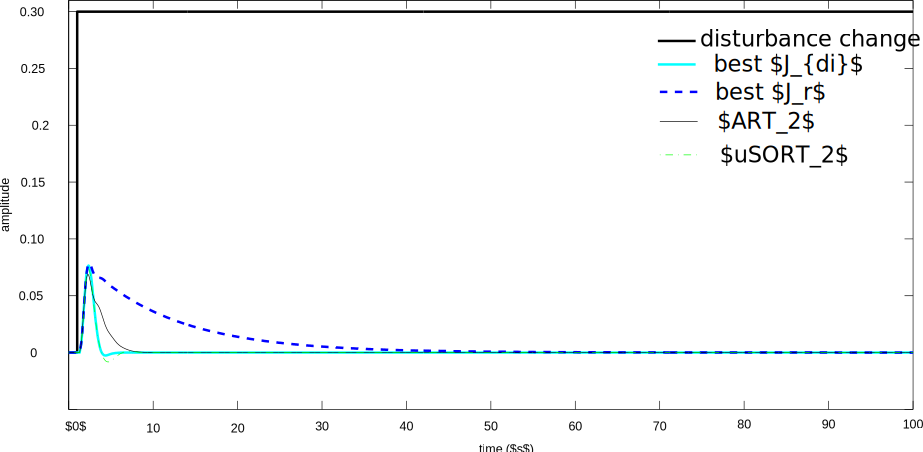
\includegraphics[width=0.9\columnwidth]{cambiodi}%
	\caption{Optimal response of the control system $J_{di}$}%
	\label{fig:cambiodi}%
\end{figure}
%
%IAE ante cambio en valor de referencia
\begin{table}[tb]
	\caption{Servo response for the benchmark system.}
	\centering
	\begin{tabular}{@{}*{3}{c}@{}}
		\toprule
		Tuning             &IAE        &$M_s$   \\
		\midrule              
		optimum $J_{r}$     &$1.004$   & $2$    \\
		optimum $J_{di}$    &$1.297$   & $2$    \\
		$uSORT_2$          &$1.522$   & $2$    \\
		$ART_2$          &$2.121$   & $2$    \\	
		\bottomrule				
	\end{tabular}
	\label{tab:IAEref}
\end{table}
%
%IAE ante cambio en perturbación
\begin{table}[tb]
	\caption{Regulator response for the benchmark system.}
	\centering
	\begin{tabular}{@{}*{3}{c}@{}}
		\toprule
		Tuning            &IAE        &$M_s$   \\
		\midrule              
		optimum $J_{di}$   &$0.1017$   & $2$    \\
		$uSORT_2$          &$0.1095$   & $2$    \\
		$ART_2$            &$0.1574$    & $2$    \\	
		optimum $J_{r}$    &$0.8283$   & $2$    \\
		\bottomrule				
	\end{tabular}
	\label{tab:IAEdi}
\end{table}
%-----------------------------------------------------------------------------------------------------------------------------------
\section{LiTaO$_3$ Thin Film Deposition Process}
\label{sec:LiTAO3}
Temperature control is a very important factor in the deposition process of lithium tantalate (LiTaO$_3$) by means of metal organic chemical vapor deposition (MOCVD) \cite{Zhang2004}.


The dynamics of the reactor chamber are characterized by a large lag and time-delay. It is important for the quality of the final product, that the controller follow a predefined temperature profile accurately (servo control) while been able to reject other disturbances (regulatory control).

The model of the MOCVD chamber can be given by:
\begin{equation}
G(s) = \frac{K e^{-L s}}{T s+1},
\label{eq:GsLita}
\end{equation}
%
where the gain $K = 3.2$, the time constant $T = 200$~s and the time-delay $L = 150$~s.

For this case, a two function MOOP is considered with $J_{di}$ and $J_{r}$ as cost functions and a robustness restriction of $M_S = 2.0$. When solving the optimization using the ENNC method, the obtained Pareto front is as given in %
\begin{figure}
	\centering
	\begin{tikzpicture}
	\begin{axis}[
	xlabel = $J_{di}$,
	ylabel = $J_{r}$,
	grid = major,
	width=0.8\columnwidth,
	xtick={0.7,0.75,...,1.2},
	ytick={1.2,1.22,...,1.5},
	]
	\addplot[mark=none, line width=2pt,] table[x=Jdi, y=Jr]{./tablas/Pareto_LiTa_ms2.dat};
	\end{axis}
	\end{tikzpicture}
	\caption{Pareto front for the LiTaO$_3$ thin film deposition process.}
	\label{fig:LitaPareto}
\end{figure}
%
figure~\ref{fig:LitaPareto}. In this case, the Pareto front is fairly convex.

\textbf{TO DO!!!!}
%-----------------------------------------------------------------------------------------------------------------------------------
%
\section{Continuous stirred tank heater}
\label{sec:CSTH}
%
\subsection{Description of the process}
\label{sec:Description}
%
The control of a \gls{csth} is a common task in industrial processes. In this section, the control of the temperature of the \gls{csth} will be solved as a \gls{moop} using a \gls{2dof} \gls{pid} controller. The diagram of the process is presented in %
\begin{figure}[b]
	\centering
	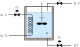
\includegraphics{Ch7CSTR}
	\caption{Simplified diagram of a continuous stirred-tank heater to be controlled.}
	\label{fig:Ch7CSTR}
\end{figure}
Figure~\ref{fig:Ch7CSTR}. A heat exchanger is installed inside the tank to heat the fluid. The flow rate inside the heat exchanger is controlled with a valve with input variable $U_T$ and the liquid inside the heat exchanger enters with temperature $T_{ci}$ and leaves with temperature $T_{co}$, the average temperature inide the heat exchanger is $T_{ca}$. The volume inside the tank is variable, the input flow rate is $Q_i$ with temperature $T_i$. The output flow rate is $Q$ with temperature $T$. The output flow rate is controlled with a valve with input variable $U_L$. The tank is covered with a jacket that prevents any heat loss to the atmosphere.

According to \cite{Alfaro2016}, a possible model for this process is given by the following set of algebraic-differential equations:
\begin{itemize}
	\item Tank mass balance:
			\begin{equation*}
				A \frac{d H(t)}{dt} = Q_i(t) - Q(t),
			\end{equation*}
			where $A$ is the transversal area of the tank and $H(t)$ is the liquid level.
	\item Tank energy balance:
			\begin{equation*}
				\rho C_p A H(t) \frac{T(t)}{dt} = \rho C_p Q_i(t)\left( T_i(t) - T(t)\right) + W(t),
			\end{equation*}
			where $C_p$ is the heat capacity of the fluid and $W(t)$ is the rate of heat transfer from the heat exchanger to the tank. $W(t)$ can be modeled as:
	\item Heat exchanger energy balance:
			\begin{equation*}
				\rho_c C_{pc} V_c \frac{T_{ca}(t)}{dt} = \rho_c C_{pc} Q_c(t)\left( T_{ci}(t)-T_{co}(t)\right) - W(t),
			\end{equation*}
			where $\rho_c$ is the density of the fluid inside the heat exchanger, $C_{pc}$ is the heat capacity of the fluid inside the heat exchanger and $V_c$ is the volume of the heat exchanger.
	\item Heat transfer between the heat exchanger and the fluid in the tank:
			\begin{equation*}
				W(t) = U A_c \left( T_{ca}(t) - T(t)\right), 
			\end{equation*}
			where $U$ is overall heat-transfer coefficient, $A_c$ is the area of the heat exchanger, $T_{ca}(t)$ is the average temperature inside the heat exchanger which is related to $T_{co}(t)$ and $T_{ci}(t)$ as:
			\begin{equation*}
				T_{ca}(t) = \frac{T_{ci}(t) + T_{co}(t)}{2}
			\end{equation*}
\end{itemize}

Also, in \cite{Alfaro2016}, the transmitters and the valves are modeled as:
\begin{itemize}
	\item Level transmitter: it is supposed that the level transmitter is a capacitive type electronic transmitter that has a first order dynamics:
		\begin{equation*}
			T_L \frac{d Y_L(t)}{dt} + Y_L(t) = K_L H(t),
		\end{equation*}
		%
		where $T_L$ is its time constant, $Y_L$ is the level signal and $K_L$ is the transmitter gain.
	%
	\item Temperature transmitter: It is supposed that a Pt$_{100}$ RTD electronic sensor is installed in a thermowell at the tank outlet pipe. It is supposed that it has a second order dynamic:
	%
		\begin{equation*}
			T_{T}^2 \frac{d^2 Y_T(t)}{dt^2} + 2T_T \frac{d Y_T(t)}{dt} + Y_T(t) = K_T T(t),
		\end{equation*}
		%
		where $T_T$ is its time constant and $K_T$ is its gain.
	%
	\item Level control valve: it is supposed that a ball valve with an electroneumatic actuator is used. The valve	inherent flow characteristics is nearly quadratic and the relationship between the flow $Q(t)$ and the input variable $U_L$ is given by:
		\begin{align*}
			T_{vL} \frac{d X_L(t)}{dt} + X_L(t) = K_{xL} U_L(t),\\
			Q(t) = K_{vL} X_L^2(t)\sqrt{\rho g H(t)},
		\end{align*}
		where $T_{vL}$ is the level control valve time constant, $K_{xL}$ level control valve stem constant $K_{vL}$ level control valve constant and $X_L(t)$ is the level control valve stem normalized travel.
	%
	\item Temperature control valve it is also supposed to be a ball valve with an electroneumatic actuator, however, it is supposed that the valve has an equal-percentage inherent flow characteristics given by:
		\begin{align*}
			T_{vT} \frac{d X_T(t)}{dt} + X_T(t) = K_{xT} U_T(t),\\
			Q_c(t) = K_{vT}R_{vT}^{\left( X_T(t) -1 \right) } \sqrt{P_{cp} - \left(R_c Q^2_c(t)+P_{cr} \right) },
		\end{align*}
		where $T_{vT}$ is the temperature control valve time constant, $K_{xT}$ the temperature control valve stem constant, $K_{vT}$ is the temperature control valve constant $P_{cp}$ is the heating fluid pump discharge pressure, $P_{cr}$ is heating fluid system return pressure and $X_T(t)$ is the temperature control valve stem normalized travel.
\end{itemize}

Taking this model in consideration, it can be said that, from the point of view of the controller, the controlled variables are give by the signals $Y_L(t)$ (which represents the level) and $Y_T(t)$ (which represents the temperature of the fluid of the tank). The manipulated variables are given by $U_L(t)$ (which directly affects $Q$) and $U_T(t)$ (that directly affects $Q_{c}$). $Q_i(t)$, $T_i$ and $T_{ci}$ are considered as disturbances. The state variables of the system are given by $H(t)$, $T_T(t)$, $T_{co}$, $Y_L(t)$, $Y_T$, $X_L(t)$ and $X_T(t)$, therefore, this model comprises a seventh order non-linear system for a two-input two-output industrial process. The parameters of the model can be found in 
\begin{table}
	\centering
	\caption{Parameters for the CSTH process}
	\label{tab:ParametersCSTH}
	\begin{tabular}{ccc}
		\toprule
		\textbf{Symbol} & \textbf{Value} & \textbf{Description}\\
		\midrule
		\multicolumn{3}{c}{\textbf{\textit{Tank parameters}}}\\
		\midrule
		$\rho$ 		& \SI{1200}{\kilogram\per\meter\cubed} 			& tank fluid density\\
		$A$			& \SI{0.0707}{\square\meter}					& tank inside section area\\
		$C_p$		& \SI{4190}{\joule\per\kilogram\per\celsius}	& tank fluid heat capacity\\
		$g$			& \SI{9.8}{\meter\per\square\second}			& gravity acceleration\\
		$K_T$		& \SI{2}{\%\per\celsius}						& temperature transmitter gain\\
		$K_{vL}$	& \num{1.25e-5}									& level control valve constant\\
		$K_{vT}$	& \num{3e-6}									& temperature control valve constant\\
		$K_{xL}$	& \SI{0.01}{\per\%}								& level control valve stem constant\\
		$Q_i$		& \SI{7e-4}{\cubic\meter\per\second}			& normal tank inlet fluid flow rate\\
		$T_i$		& \SI{24}{\celsius}								& fluid inlet temperature\\
		$T_L$		& \SI{2}{\second}								& level transmitter time constant\\
		$T_T$		& \SI{15}{\second}								& temperature transmitter time constant\\
		$T_{vL}$	& \SI{3}{\second}								& level control valve time constant\\
		$T_{vT}$	& \SI{5}{\second}								& temperature control valve time constant\\
		\midrule
		\multicolumn{3}{c}{\textbf{\textit{Heat exchanger parameters}}}\\
		\midrule
		$\rho_c$ 	& \SI{800}{\kilogram\per\meter\cubed} 			& heating fluid density\\
		$A_c$		& \SI{0.6362}{\square\meter}					& heat exchanger transfer area\\
		$C_{pc}$	& \SI{2400}{\joule\per\kilogram\per\celsius}	& heating fluid heat capacity\\
		$K_L$		& \SI{125}{\%\per\meter}						& level transmitter gain\\
		$K_{xT}$	& \SI{0.01}{\per\%}								& temperature control valve stem constant\\
		$P_{cp}$	& \SI{4.14e5}{\pascal}							& heating fluid pump discharge pressure\\
		$P_{cr}$	& \SI{1.38e5}{\pascal}							& heating fluid system return pressure\\
		$R_c$		& \SI{5.5e10}{\pascal\per(\cubic\meter\per\second)^2}	& heating system pipe nominal flow resistance\\
		$R_{vT}$	& \num{50}										& temperature control valve rangeability\\
		$T_{ci}$	& \SI{320}{\celsius}							& heating fluid inlet temperature\\
		$U$			& \SI{440}{\joule\per\second\per\square\meter\per\celsius}	& overall heat-transfer coefficient\\
		$V_c$		& \SI{0.0139}{\cubic\meter}						& heat exchanger volume\\
		\bottomrule
	\end{tabular}
\end{table}
%
Table~\ref{tab:ParametersCSTH}. This model was implemented in Simulink and can be found with the companion software. In %
%
\begin{figure}[tb]
	\centering
	\includegraphics[width=\columnwidth]{Ch7Implementation}
	\caption{Simulink implementation of the model of the heater.}
	\label{fig:Ch7Implementation}
\end{figure}
%
Figure~\ref{fig:Ch7Implementation}. Each equation of the model was implemented in a subsystem for clarity. For example in %
\begin{figure}
	\centering
	\includegraphics[width=\columnwidth]{Ch7HeatExhangerEq}
	\caption{Example of the implementation of the heat exchanger energy balance.}
	\label{fig:Ch7HeatExhangerEq}
\end{figure}
%
Figure~\ref{fig:Ch7HeatExhangerEq} the Simulink implementation of the heat exchanger energy balance is presented. The result of this submodel is the computation of the state variable $T_{ca}$, which represents the average temperature of the heating fluid. As it can be seen, the parameters of the model are not hard-coded in the Simulink blocks, instead a parameter initialization script is call before the simulation starts. If the user desires to change any value of the parameters, it can be done globally in the script and then automatically called during the simulation.

\subsection{Simplified linear model}
\label{sec:SimpLinMod}
In order to find a PID controller using the MOOTuning app, it is necessary to find a linear model of the plant in the operation point. An identification procedure was performed with a change of 10\% in the value of $U_T$ to find the transfer function between $Y_T$ and $U_T$. The response to this change is depicted in %
\begin{figure}[tb]
	\centering
	\includegraphics[width=0.8\columnwidth]{Ch7CSTHResp}
	\caption{Response of the process to a change of 10\% in the $U_T(t)$ input.}
	\label{fig:Ch7CSTHResp}
\end{figure}
%
Figure~\ref{fig:Ch7CSTHResp}. As it can be seen, the response is overdamped and takes approximately \SI{500}{\second} to reach a new steady state. A change in 10\% on the input signal produces a variation of approximately $3.5\%$ in the output signal. It has to be noticed that the presented signals are normalized between 0 and 100\% representing the full spam of the transmitter and actuators.

In order to find the model, the process was supposed to have two poles, no zeros and a pure time-delay (also known as dead-time). Of course, if a linearization procedure were performed using the nonlinear model, a seventh order model would be obtained. However, for PID tuning, a first or second order model is usually expected to tune the controller.

Considering the experiment performed with the data as depicted in Figure~\ref{fig:Ch7CSTHResp}, the resulting simplified model is given by:
%
\begin{equation}
\frac{Y_T(s)}{U_T(s)} = \frac{0.3658 e^{-24.736 s}}{(52.861 s+1)(52.805 s +1)}.
\label{eq:TFCSTH}
\end{equation}

From this transfer function, it can be deduced that the gain is equal to $K = 0.3658$, the main time constant is given by $T = 52.861$, the ratio between the two time constant is given by $a = 0.9989$ and the dead-time is given by $L = 24.736$, therefore the normalized dead-time is given by $\tau = 0.4679$.

To test the validity of this simplified model, the response of the transfer function is compared against the response of the non-linear model. It was found that the transfer function response is very similar to the response of the non-linear model, as can be seen in %
%
\begin{figure}[tb]
	\centering
	\includegraphics[width=\columnwidth]{Ch7CSTHComp}
	\caption{Comparison between the linear and no linear models for the CSTH.}
	\label{fig:Ch7CSTHComp}
\end{figure}
%
Figure~\ref{fig:Ch7CSTHComp}. It is clear that the non-linear model is a good representation of the dynamical response of the process. This is the first step in order to find a suitable PID controller to control the plant. In \cite{Alfaro2016} the level of the tank is also controlled, however the dynamic of the level is simpler (its model can be approximated with a first order model without delay) and in this particular example, only the temperature is going to be controlled, while the level is considered to be constant.
%
\subsection{PID control of the CSTH}
\label{sec:PIDCSTH}
In this section, the process will be controlled using a \gls{pid} controller with different tuning methods and compared with the \gls{moo} framework used in the book.

Two different tuning rules were considered: the method by Rovira~\cite{Rovira1969a} and the method by Murril~\cite{Murril1967}. For the case of the Rovira and Murril method, the model in \eqref{eq:TFCSTH} was reduced to a first order model using the Half-Rule in \cite{Skogestad2003}:
\begin{equation}
\frac{Y_T(s)}{U_T(s)} = \frac{0.3658 e^{-24.7360 s}}{79.2635 s +1}.
\label{eq:TFCSTHFirstOrder}
\end{equation}

The equations were implemented as presented in \cite{odwyer2006}:
\begin{itemize}
%	\item SIMC method: Supposing a \gls{soptd} model:
%			\begin{equation*}
%				P(s) = \frac{K e^{-Ls}}{(Ts+1)(aTs+1)}
%			\end{equation*}
%			The corresponding PID tuning for a closed-loop lag time of $T_c = L$ and the case where $T \leq 8 L$, the PID tuning is given by:
%			\begin{align*}
%				K_p &= \frac{0.5}{K}\frac{(1+a)T}{L}\\
%				T_i &= (1 + a) T\\
%				T_d	&= \frac{a}{1+a}T
%			\end{align*}
%	%
	\item Supposing a \gls{foptd} model given by:
			\begin{equation*}
				P(s) = \frac{K e^{-L s}}{Ts+1}
			\end{equation*}
			The Murrill tuning is given by:
				\begin{align*}
					K_p &= \frac{1.435}{K}\left( \frac{T}{L} \right)^{0.921}\\
					T_i &= \frac{T}{0.878}\left( \frac{L}{T}\right)^{0.749}\\\\
					T_d &= 0.482 T \left( \frac{L}{T} \right)^{1.137}
				\end{align*}
	\item Again, supposing a \gls{foptd} as above, the Rovira tuning is given by:
			\begin{align*}
				K_p &= \frac{1.086}{K} \left( \frac{T}{L}\right) ^{0.869} \\
				T_i &= \frac{T}{0.740 - 0.13\frac{L}{T}} \\
				T_d &= 0.384 T \left( \frac{L}{T}\right)^{0.914} 
			\end{align*}
\end{itemize}

The values of the computed values can be found on %
\begin{table}[tb]
	\centering
	\caption{Comparison of different PID tunings for the CSTH process.}
	\setlength{\tabcolsep}{8pt}
	\begin{tabular}{ccccccc}
		\toprule
		Tuning 	& $K_p$ 	& $T_i$		& $T_d$		& $\beta$	& $J_{r}$	& $J_{di}$\\
		\midrule
		%
		%SIMC	& $5.84$	& $105.67$	& $26.42$	& $1$			& $55.14$	& $18.10$\\
		Murril	& $5.87$	& $65.02$	& $23.21$	& $1$			& $82.51$	& $15.34$\\
		Rovira	& $4.34$	& $120.81$	& $18.48$	& $1$			& $76.00$	& $27.79$\\
		MOO01	& $11.3$	& $58.82$	& $29.48$	& $0.43$		& $85.65$	& $7.06$\\
		MOO02	& $9.26$	& $123.85$	& $26.68$	& $0.80$		& $69.96$	& $13.38$\\
		MOO03	& $8.20$	& $185.21$	& $28.14$	& $0.99$		& $67.93$	& $22.54$\\
		\bottomrule
	\end{tabular}
	\label{tab:CompPIDCSTH}
\end{table}
%
Table~\ref{tab:CompPIDCSTH}, along with its associated values of $J_{di}$ and $J_r$. The Murril and Rovira methods presented in the table were selected because they are intended to minimize the \gls{iae}. The SIMC method was selected because it presents a good compromise between performance, robustness and easiness of the tuning rule. In all cases, the PID tuning is for a one degree of freedom controller (that is  the reason why $\beta$ is equal to one).

The PID that can be found using the data and the framework presented in Chapter~\ref{chap:PIDMOOP} is a \gls{soptd}, which may do the comparison somehow unfair. However, below another comparison is made using the same controller topology, the idea now is to compare methods that tries to minimize the \gls{iae}. Using the MOOTuning Tool that accompanies this book, the Pareto front that was found is given as in %
%
\begin{figure}[tb]
	\centering
	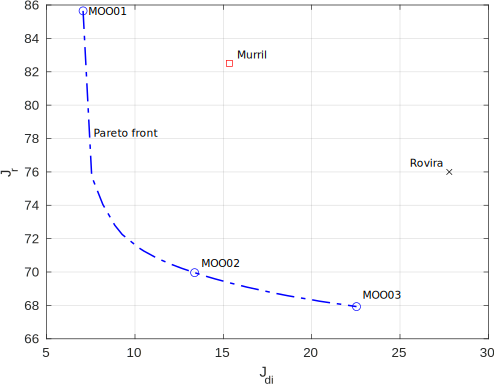
\includegraphics[width=0.8\columnwidth]{Ch7CompPareto}
	\caption{MOOTuning compared to the Murril and Rovira methods that also minimizes \gls{iae}.}
	\label{fig:Ch7CompPareto}
\end{figure}
%
Figure~\ref{fig:Ch7CompPareto}. As it was expected, all the controllers found using the \gls{moo} tool present lower values for $J_{di}$ and $J_r$. If all controllers had the same topology, most certainly both controller would be close to the anchor points. However, what it is important here is the fact that, using the tool, the user has the ability to chose between practically an infinity of possible controllers. From the Pareto front, three different tuning were selected in order to compare the responses using the non-linear plant. The values of the parameters are presented also in Table~\ref{tab:CompPIDCSTH} and depicted as circles in the Pareto front in Figure~\ref{fig:Ch7CompPareto}.
%
\begin{figure}[tb]
	\centering
	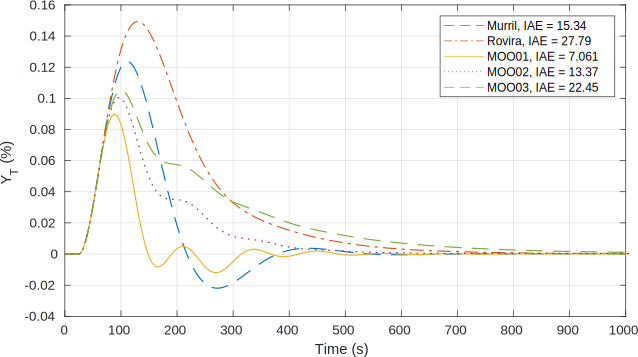
\includegraphics[width=0.8\columnwidth]{Ch7CompParetoReg}
	\caption{Regulator response comparison for minimum IAE.}
	\label{fig:Ch7CompParetoReg}
\end{figure}
%
\begin{figure}[tb]
	\centering
	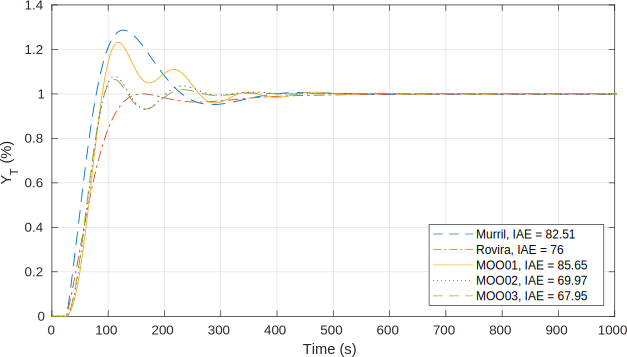
\includegraphics[width=0.8\columnwidth]{Ch7CompParetoServo}
	\caption{Servo response comparison for minimum IAE.}
	\label{fig:Ch7CompParetoServo}
\end{figure}

In Figures~\ref{fig:Ch7CompParetoReg} and \ref{fig:Ch7CompParetoServo} the responses to a step change in the setpoint and in the disturbance are presented. The corresponding values of \gls{iae} are also presented in the graph. In all cases, the robustness was not considered as a constraint. but it is possible to include it within the MOOTuning software. From Figure~\ref{fig:Ch7CompPareto} given the steep slope of the curve for lower values of $J_{di}$ that a small change in $J_{di}$ may improve substantially the performance for $J_r$. Therefore, one may be more prone to select a controller that may have a little degradation in $J_{di}$ and for this reason, controller MOO01 may not be a good selection as a final solution unless having the minimum value possible of $J_{di}$ is the final goal.

The controller MOO02 may be seen as an intermediate solution between MOO1 and MOO03 in case both $J_{di}$ and $J_r$ are equally important for the decision maker. The power of the multiobjective framework is evident, and giving that the computational power is done offline, it becomes a good tool for the tuning of PIDs in an industrial setting.

\textbf{TO DO!!!!}
\backmatter%%%%%%%%%%%%%%%%%%%%%%%%%%%%%%%%%%%%%%%%%%%%%%%%%%%%%%%
\input{./backmatter/glossary}
%\include{solutions}
%\printindex
\bibliographystyle{spmpsci}
\bibliography{ReferenciasMulti}

%%%%%%%%%%%%%%%%%%%%%%%%%%%%%%%%%%%%%%%%%%%%%%%%%%%%%%%%%%%%%%%%%%%%%%

\end{document}





